
\documentclass[
	% -- opções da classe memoir --
	12pt,				% tamanho da fonte
	openright,			% capítulos começam em pág ímpar (insere página vazia caso preciso)
	twoside,			% para impressão em verso e anverso. Oposto a oneside
	a4paper,			% tamanho do papel. 
	% -- opções da classe abntex2 --
	%chapter=TITLE,		% títulos de capítulos convertidos em letras maiúsculas
	%section=TITLE,		% títulos de seções convertidos em letras maiúsculas
	%subsection=TITLE,	% títulos de subseções convertidos em letras maiúsculas
	%subsubsection=TITLE,% títulos de subsubseções convertidos em letras maiúsculas
	% -- opções do pacote babel --
	english,			% idioma adicional para hifenização
	french,				% idioma adicional para hifenização
	spanish,			% idioma adicional para hifenização
	brazil,				% o último idioma é o principal do documento
	]{abntex2}

\usepackage{cmap}			% Mapear caracteres especiais no PDF
\usepackage{lmodern}			% Usa a fonte Latin Modern			
\usepackage[T1]{fontenc}		% Selecao de codigos de fonte.
\usepackage[utf8]{inputenc}		% Codificacao do documento (conversão automática dos acentos)
\usepackage{lastpage}			% Usado pela Ficha catalográfica
\usepackage{indentfirst}		           % Indenta o primeiro parágrafo de cada seção.
\usepackage{color}				% Controle das cores
\usepackage{graphicx}			% Inclusão de gráficos
\usepackage{lipsum}			% para geração de dummy text

\usepackage[brazilian,hyperpageref]{backref}   % Paginas com as citações na bibl
\usepackage[alf]{abntex2cite}	                         % Citações padrão ABNT
% Configurações do pacote backref
% Usado sem a opção hyperpageref de backref
\renewcommand{\backrefpagesname}{Citado na(s) página(s):~}
% Texto padrão antes do número das páginas
\renewcommand{\backref}{}
% Define os textos da citação
\renewcommand*{\backrefalt}[4]{
	\ifcase #1 %
		Nenhuma citação no texto.%
	\or
		Citado na página #2.%
	\else
		Citado #1 vezes nas páginas #2.%
	\fi}%
% ---


% ---
% Informações de dados para CAPA e FOLHA DE ROSTO
% ---
\titulo{Modelo de Monografia de \\ Trabalho de Conclusão de Curso com \abnTeX}
\autor{<Nome Completo do Aluno>}
\local{Belo Horizonte}
\data{2013}
\orientador{Prof. <Nome Completo do Orientador>}
%\coorientador{Prof. }
\instituicao{%
  Universidade Federal de Minas Gerais -- UFMG
  \par
  Escola de Engenharia
  \par
  Curso de Graduação em Engenharia Elétrica}
\tipotrabalho{Trabalho de Conclusão de Curso}
% O preambulo deve conter o tipo do trabalho, o objetivo, o nome da instituição e a área de concentração 
\preambulo{Monografia apresentada durante o Seminário dos Trabalhos de Conclusão do Curso de Graduação em Engenharia Elétrica da UFMG, como parte dos requisitos necessários à obtenção do título de Engenheiro Eletricista.}
% alterando o aspecto da cor azul
\definecolor{blue}{RGB}{41,5,195}

% informações do PDF
\makeatletter
\hypersetup{
     	%pagebackref=true,
		pdftitle={\@title}, 
		pdfauthor={\@author},
    	pdfsubject={\imprimirpreambulo},
	    pdfcreator={LaTeX with abnTeX2},
		pdfkeywords={abnt}{latex}{abntex}{abntex2}{trabalho acadêmico}, 
		colorlinks=true,       	% false: boxed links; true: colored links
    	linkcolor=blue,          	           % color of internal links
    	citecolor=blue,        		% color of links to bibliography
    	filecolor=magenta,      		% color of file links
		urlcolor=blue,
		bookmarksdepth=4
}
\makeatother
% O tamanho do parágrafo é dado por:
\setlength{\parindent}{1.3cm}

% Controle do espaçamento entre um parágrafo e outro:
\setlength{\parskip}{0.2cm}  % tente também \onelineskip
\makeindex

% Início do documento
% ----
\begin{document}
% Retira espaço extra obsoleto entre as frases.
\frenchspacing 
%\imprimircapa
%\imprimirfolhaderosto

%
\begin{dedicatoria}
   \vspace*{\fill}
   \centering
   \noindent
   \textit{ Este trabalho é dedicado às crianças adultas que,\\
   quando pequenas, sonharam em se tornar cientistas.} \vspace*{\fill}
\end{dedicatoria}
\begin{agradecimentos}
\end{agradecimentos}

\begin{epigrafe}
    \vspace*{\fill}
	\begin{flushright}
		\textit{``Não vos amoldeis às estruturas deste mundo, \\
		mas transformai-vos pela renovação da mente, \\
		a fim de distinguir qual é a vontade de Deus: \\
		o que é bom, o que Lhe é agradável, o que é perfeito.\\
		(Bíblia Sagrada, Romanos 12, 2)}
	\end{flushright}
\end{epigrafe}
% ---

% ---
% RESUMOS
% ---
% resumo em português
\setlength{\absparsep}{18pt} % ajusta o espaçamento dos parágrafos do resumo
\begin{resumo}

 objetivo, o método, os resultados e as conclusões do documento. A ordem e a extensão
 destes itens dependem do tipo de resumo (informativo ou indicativo) e do
 tratamento que cada item recebe no documento original. O resumo deve ser
 precedido da referência do documento, com exceção do resumo inserido no
 próprio documento. (\ldots) As palavras-chave devem figurar logo abaixo do
 resumo, antecedidas da expressão Palavras-chave:, separadas entre si por
 ponto e finalizadas também por ponto.

 \textbf{Palavras-chaves}: latex. abntex. editoração de texto.
\end{resumo}

% resumo em inglês
\begin{resumo}[Abstract]
 \begin{otherlanguage*}{english}
   This is the english abstract.

   \vspace{\onelineskip}
 
   \noindent 
   \textbf{Key-words}: latex. abntex. text editoration.
 \end{otherlanguage*}
\end{resumo}

% ---
% inserir lista de ilustrações
% ---
\pdfbookmark[0]{\listfigurename}{lof}
\listoffigures*
\cleardoublepage
% ---

% ---
% inserir lista de tabelas
% ---
\pdfbookmark[0]{\listtablename}{lot}
\listoftables*
\cleardoublepage
% ---

% ---
% inserir lista de abreviaturas e siglas
% ---
\begin{siglas}
  \item[Fig.] Area of the $i^{th}$ component
  \item[456] Isto é um número
  \item[123] Isto é outro número
%  \item[lauro cesar] este é o meu nome
\end{siglas}
% ---

% ---
% inserir lista de símbolos
% ---
\begin{simbolos}
  \item[$ \Gamma $] Letra grega Gama
  \item[$ \Lambda $] Lambda
  \item[$ \zeta $] Letra grega minúscula zeta
  \item[$ \in $] Pertence
\end{simbolos}
% ---

% ---
% inserir o sumario
% ---
\pdfbookmark[0]{\contentsname}{toc}
\tableofcontents*
\cleardoublepage
% ---

% ----------------------------------------------------------
% ELEMENTOS TEXTUAIS
% ----------------------------------------------------------
\textual

% ----------------------------------------------------------
% Capítulo 1 - Introdução
% ----------------------------------------------------------


\chapter{Introdução}
 
A atual arquitetura de rede da Internet é composta por: nós de comutação (roteadores e switches, responsáveis pelo encaminhamento de pacotes de dados) e os hosts (máquinas de origem e destino de pacotes de dados, como computadores de usuários, servidores, smartphones, etc). Os nós de comutação possuem uma tabela que os indica qual é o próximo nó que um pacote deve ser encaminhado , chamada de tabela de encaminhamento. Como um pacote pode passar por múltiplos nós até chegar ao seu destino, e como o fluxo de pacotes em cada nó é extremamente alto, toda a operação de consulta a tabela de encaminhamento e transmissão de dados é realizado via hardware. Como o exemplo (Figura \ref{Fig_Rede}) onde observa-se uma rede de Internet de maneira simplificada .

\begin{figure}[h]
\centering
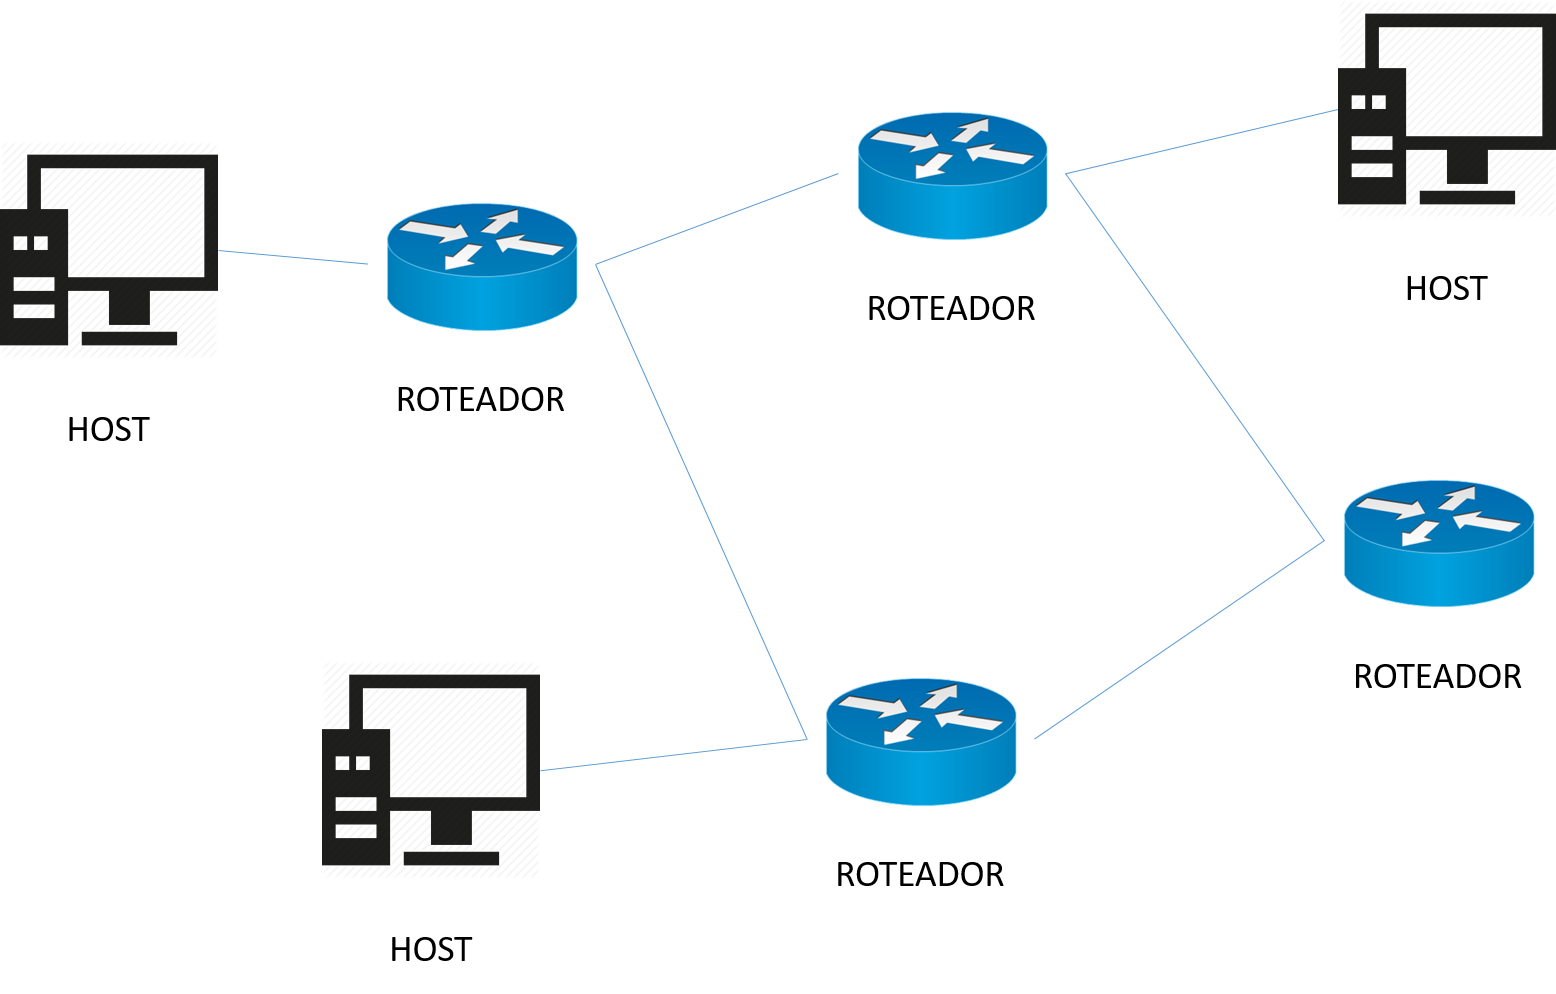
\includegraphics[width=0.7\textwidth]{Introducao/Rede.png}
\caption{Estrutura de uma Rede}
\label{Fig_Rede}
\end{figure}

Essa estrutura se mostrou extremamente eficiente, e permitiu que a expansão em nível mundial da Internet, uma vez que diversas redes com tamanhos e topologias diferentes conseguem se comunicar. 

Proporcional à expansão da Internet e a criação de cada vez mais dispositivos capazes de usá-la, houve um grande aumento no fluxo de dados. Tal aumento advém de práticas como o consumo de vídeo, através de plataformas como Youtube, Netflix, etc, sendo este o tipo de dado mais consumido e o segundo que mais cresce desde 2017\cite{CISCO}

Portanto, devido a essa progressiva demanda, novas arquiteturas de rede estão sendo investigadas. Contudo, como o núcleo da arquitetura atual, ou seja, os nós de comutação, são implementados via hardware, a implementação de arquiteturas experimentais se torna pouco viável, devido aos grandes custos dessa mudança de hardware, além do fato que essa troca iria interromper o fluxo de produção atual de uma rede, fator que dificulta o teste e validação de novas arquiteturas em ambientes reais, principalmente em redes de larga escala.

Dessa forma, soluções baseadas em software se tornaram mais atraentes devido a possibilidade de serem implementadas sem troca de hardware e sem interrupção da rede. Uma dessas alternativas que tem ganhado destaque é o paradigma SDN(Software Defined NetWork) juntamente com o protocolo OpenFlow. Uma rede SDN, utiliza de um dispositivo chamado controlador, que se conecta a todos os nós da rede, para configurá-los de acordo com o gerente da rede. O protocolo Openflow é um protocolo voltado para as redes SDN, que permite que o controlador se comunique com os comutatores.

A implementação de redes SDN ainda está numa fase experimental, e por isso, diversas pesquisas estão sendo desenvolvidas para verificar a performance desse tipo de rede. Uma das grandes vantagens de uma rede SDN é a possibilidade de separar o tráfego de dados em fluxos diferentes, além de poder alterar a tabela de encaminhamento dos comutatores para atingir um melhor desempenho da rede. 

Dessa forma, o objetivo desse trabalho é a criação de uma aplicação capaz de monitorar o fluxo de uma rede e identificar o consumo de dados de vídeos, provenientes de duas das principais plataformas de streaming : Youtube e NetFlix. Essa aplicação será integrada a um tipo de controlador chamado POX e testada através de software capaz de simular redes fisicas, chamado Mininet. Os conceitos de SDN , protocolo OpenFlow e controlador POX serão explicados de forma mais detalhada no capítulo 2.

\section{Objetivos}
\subsection{Objetivo geral}
Implementar e avaliar o desempenho de uma aplicação de monitoramento e classificação de fluxos de dados, utilizando uma rede SDN , junto com um controlador do tipo POX.

\subsection{Objetivos Específicos}

\begin{itemize}
\item Criar e configurar um ambiente de rede SDN, onde seja possível gerar e capturar todo o tráfego da rede. 
\item Implementar um módulo de monitoramento do tráfego da rede, para análise posterior.
\item Implementar o módulo de identificação e classificação do tipo de dados que trafega pela rede.
\item Implementar um módulo de detecção e tratamento de falhas na rede, para que a aplicação possa priorizar um determino tipo de fluxo.
\item Utilizar um banco da dados SQL, para armazenar todos os dados gerados pela aplicação
\end{itemize}3
\section{Estrutura do Trabalho}
Este trabalho será estruturado em 5 capítulos. No capítulo 2 serão explicados mais profundamente os conceitos de paradigma SDN, protoloco OpenFlow, controlador POX, além de das estruturas da arquitetura atual da Internet. Os módulos criados para a aplicação, suas funcionalidades, especificações, e ferramentas utilizadas serão apresentados no capitulo 3, assim como o ambiente em que o módulo foi testado.

O capítulo 4 será feita uma exposição e análise dos resultados obtidos. E por fim, no capítulo 5 serão expostas as conclusões, considerações finais e trabalhos futuros.




\documentclass[
	% -- opções da classe memoir --
	12pt,				% tamanho da fonte
	openright,			% capítulos começam em pág ímpar (insere página vazia caso preciso)
	twoside,			% para impressão em verso e anverso. Oposto a oneside
	a4paper,			% tamanho do papel. 
	% -- opções da classe abntex2 --
	%chapter=TITLE,		% títulos de capítulos convertidos em letras maiúsculas
	%section=TITLE,		% títulos de seções convertidos em letras maiúsculas
	%subsection=TITLE,	% títulos de subseções convertidos em letras maiúsculas
	%subsubsection=TITLE,% títulos de subsubseções convertidos em letras maiúsculas
	% -- opções do pacote babel --
	english,			% idioma adicional para hifenização
	french,				% idioma adicional para hifenização
	spanish,			% idioma adicional para hifenização
	brazil,				% o último idioma é o principal do documento
	]{abntex2}

\usepackage{cmap}			% Mapear caracteres especiais no PDF
\usepackage{lmodern}			% Usa a fonte Latin Modern			
\usepackage[T1]{fontenc}		% Selecao de codigos de fonte.
\usepackage[utf8]{inputenc}		% Codificacao do documento (conversão automática dos acentos)
\usepackage{lastpage}			% Usado pela Ficha catalográfica
\usepackage{indentfirst}		           % Indenta o primeiro parágrafo de cada seção.
\usepackage{color}				% Controle das cores
\usepackage{graphicx}			% Inclusão de gráficos
\usepackage{lipsum}			% para geração de dummy text

\usepackage[brazilian,hyperpageref]{backref}   % Paginas com as citações na bibl
\usepackage[alf]{abntex2cite}	                         % Citações padrão ABNT
% Configurações do pacote backref
% Usado sem a opção hyperpageref de backref
\renewcommand{\backrefpagesname}{Citado na(s) página(s):~}
% Texto padrão antes do número das páginas
\renewcommand{\backref}{}
% Define os textos da citação
\renewcommand*{\backrefalt}[4]{
	\ifcase #1 %
		Nenhuma citação no texto.%
	\or
		Citado na página #2.%
	\else
		Citado #1 vezes nas páginas #2.%
	\fi}%
% ---


% ---
% Informações de dados para CAPA e FOLHA DE ROSTO
% ---
\titulo{Modelo de Monografia de \\ Trabalho de Conclusão de Curso com \abnTeX}
\autor{<Nome Completo do Aluno>}
\local{Belo Horizonte}
\data{2013}
\orientador{Prof. <Nome Completo do Orientador>}
%\coorientador{Prof. }
\instituicao{%
  Universidade Federal de Minas Gerais -- UFMG
  \par
  Escola de Engenharia
  \par
  Curso de Graduação em Engenharia Elétrica}
\tipotrabalho{Trabalho de Conclusão de Curso}
% O preambulo deve conter o tipo do trabalho, o objetivo, o nome da instituição e a área de concentração 
\preambulo{Monografia apresentada durante o Seminário dos Trabalhos de Conclusão do Curso de Graduação em Engenharia Elétrica da UFMG, como parte dos requisitos necessários à obtenção do título de Engenheiro Eletricista.}
% alterando o aspecto da cor azul
\definecolor{blue}{RGB}{41,5,195}

% informações do PDF
\makeatletter
\hypersetup{
     	%pagebackref=true,
		pdftitle={\@title}, 
		pdfauthor={\@author},
    	pdfsubject={\imprimirpreambulo},
	    pdfcreator={LaTeX with abnTeX2},
		pdfkeywords={abnt}{latex}{abntex}{abntex2}{trabalho acadêmico}, 
		colorlinks=true,       	% false: boxed links; true: colored links
    	linkcolor=blue,          	           % color of internal links
    	citecolor=blue,        		% color of links to bibliography
    	filecolor=magenta,      		% color of file links
		urlcolor=blue,
		bookmarksdepth=4
}
\makeatother
% O tamanho do parágrafo é dado por:
\setlength{\parindent}{1.3cm}

% Controle do espaçamento entre um parágrafo e outro:
\setlength{\parskip}{0.2cm}  % tente também \onelineskip
\makeindex

% Início do documento
% ----
\begin{document}
% Retira espaço extra obsoleto entre as frases.
\frenchspacing 
%\imprimircapa
%\imprimirfolhaderosto

%
\begin{dedicatoria}
   \vspace*{\fill}
   \centering
   \noindent
   \textit{ Este trabalho é dedicado às crianças adultas que,\\
   quando pequenas, sonharam em se tornar cientistas.} \vspace*{\fill}
\end{dedicatoria}
\begin{agradecimentos}
\end{agradecimentos}

\begin{epigrafe}
    \vspace*{\fill}
	\begin{flushright}
		\textit{``Não vos amoldeis às estruturas deste mundo, \\
		mas transformai-vos pela renovação da mente, \\
		a fim de distinguir qual é a vontade de Deus: \\
		o que é bom, o que Lhe é agradável, o que é perfeito.\\
		(Bíblia Sagrada, Romanos 12, 2)}
	\end{flushright}
\end{epigrafe}
% ---

% ---
% RESUMOS
% ---
% resumo em português
\setlength{\absparsep}{18pt} % ajusta o espaçamento dos parágrafos do resumo
\begin{resumo}

 objetivo, o método, os resultados e as conclusões do documento. A ordem e a extensão
 destes itens dependem do tipo de resumo (informativo ou indicativo) e do
 tratamento que cada item recebe no documento original. O resumo deve ser
 precedido da referência do documento, com exceção do resumo inserido no
 próprio documento. (\ldots) As palavras-chave devem figurar logo abaixo do
 resumo, antecedidas da expressão Palavras-chave:, separadas entre si por
 ponto e finalizadas também por ponto.

 \textbf{Palavras-chaves}: latex. abntex. editoração de texto.
\end{resumo}

% resumo em inglês
\begin{resumo}[Abstract]
 \begin{otherlanguage*}{english}
   This is the english abstract.

   \vspace{\onelineskip}
 
   \noindent 
   \textbf{Key-words}: latex. abntex. text editoration.
 \end{otherlanguage*}
\end{resumo}

% ---
% inserir lista de ilustrações
% ---
\pdfbookmark[0]{\listfigurename}{lof}
\listoffigures*
\cleardoublepage
% ---

% ---
% inserir lista de tabelas
% ---
\pdfbookmark[0]{\listtablename}{lot}
\listoftables*
\cleardoublepage
% ---

% ---
% inserir lista de abreviaturas e siglas
% ---
\begin{siglas}
  \item[Fig.] Area of the $i^{th}$ component
  \item[456] Isto é um número
  \item[123] Isto é outro número
%  \item[lauro cesar] este é o meu nome
\end{siglas}
% ---

% ---
% inserir lista de símbolos
% ---
\begin{simbolos}
  \item[$ \Gamma $] Letra grega Gama
  \item[$ \Lambda $] Lambda
  \item[$ \zeta $] Letra grega minúscula zeta
  \item[$ \in $] Pertence
\end{simbolos}
% ---

% ---
% inserir o sumario
% ---
\pdfbookmark[0]{\contentsname}{toc}
\tableofcontents*
\cleardoublepage
% ---

% ----------------------------------------------------------
% ELEMENTOS TEXTUAIS
% ----------------------------------------------------------
\textual

% ----------------------------------------------------------
% Capítulo 1 - Introdução
% ----------------------------------------------------------


\chapter{Introdução}
 
A atual arquitetura de rede da Internet é composta por: nós de comutação (roteadores e switches, responsáveis pelo encaminhamento de pacotes de dados) e os hosts (máquinas de origem e destino de pacotes de dados, como computadores de usuários, servidores, smartphones, etc). Os nós de comutação possuem uma tabela que os indica qual é o próximo nó que um pacote deve ser encaminhado , chamada de tabela de encaminhamento. Como um pacote pode passar por múltiplos nós até chegar ao seu destino, e como o fluxo de pacotes em cada nó é extremamente alto, toda a operação de consulta a tabela de encaminhamento e transmissão de dados é realizado via hardware. Como o exemplo (Figura \ref{Fig_Rede}) onde observa-se uma rede de Internet de maneira simplificada .

\begin{figure}[h]
\centering
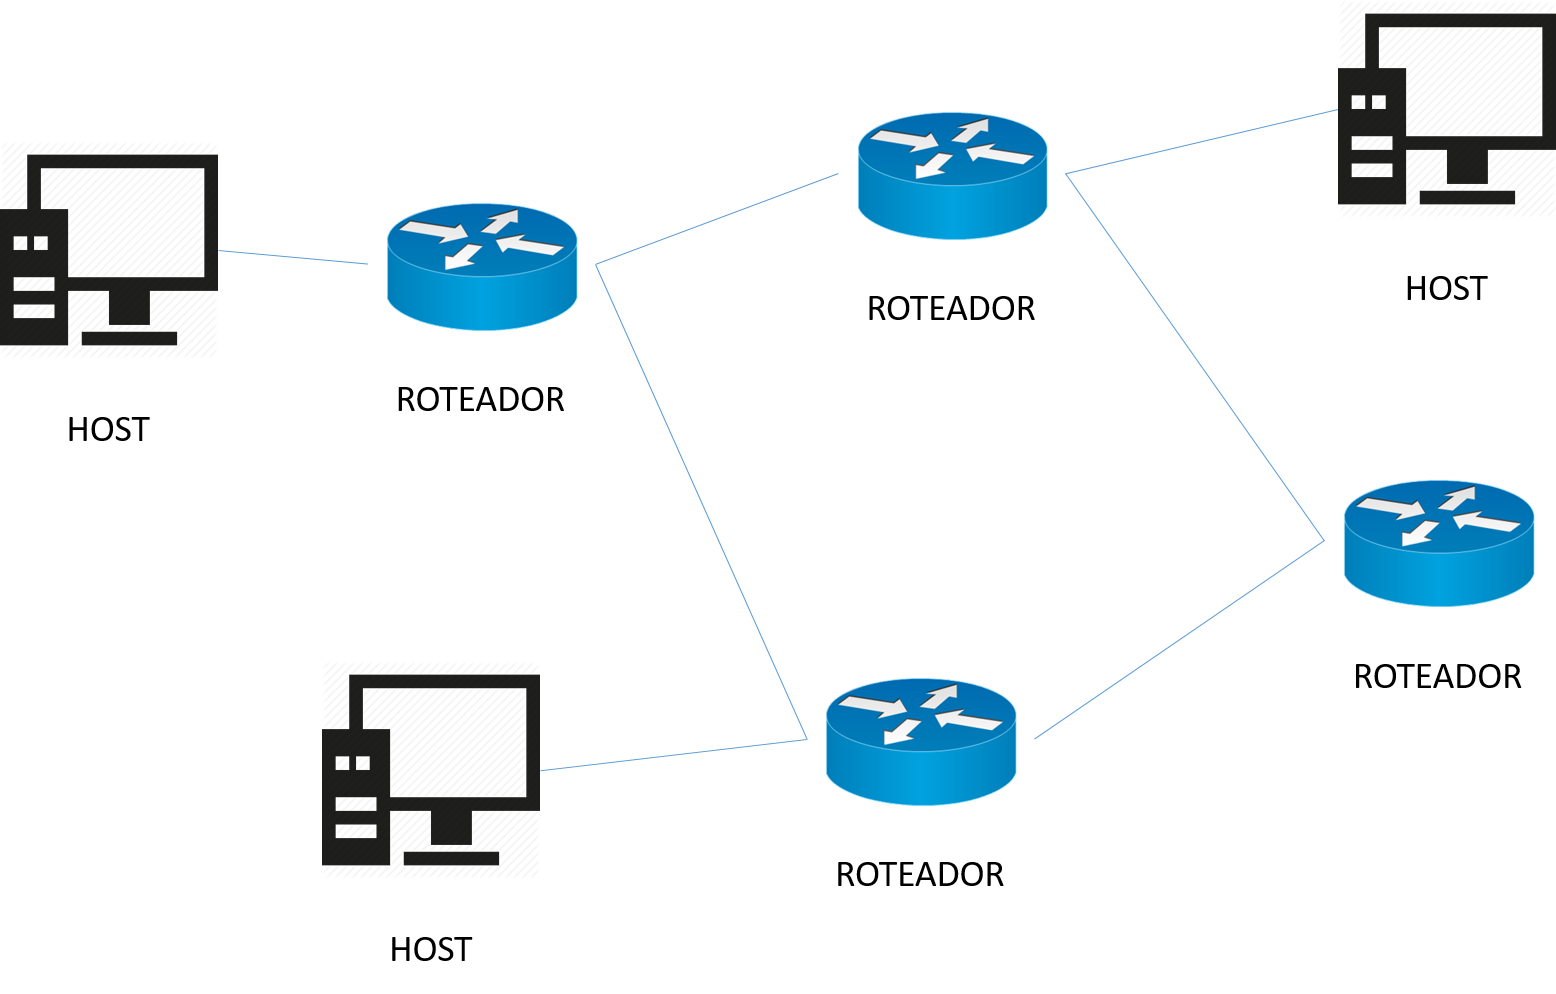
\includegraphics[width=0.7\textwidth]{Introducao/Rede.png}
\caption{Estrutura de uma Rede}
\label{Fig_Rede}
\end{figure}

Essa estrutura se mostrou extremamente eficiente, e permitiu que a expansão em nível mundial da Internet, uma vez que diversas redes com tamanhos e topologias diferentes conseguem se comunicar. 

Proporcional à expansão da Internet e a criação de cada vez mais dispositivos capazes de usá-la, houve um grande aumento no fluxo de dados. Tal aumento advém de práticas como o consumo de vídeo, através de plataformas como Youtube, Netflix, etc, sendo este o tipo de dado mais consumido e o segundo que mais cresce desde 2017\cite{CISCO}

Portanto, devido a essa progressiva demanda, novas arquiteturas de rede estão sendo investigadas. Contudo, como o núcleo da arquitetura atual, ou seja, os nós de comutação, são implementados via hardware, a implementação de arquiteturas experimentais se torna pouco viável, devido aos grandes custos dessa mudança de hardware, além do fato que essa troca iria interromper o fluxo de produção atual de uma rede, fator que dificulta o teste e validação de novas arquiteturas em ambientes reais, principalmente em redes de larga escala.

Dessa forma, soluções baseadas em software se tornaram mais atraentes devido a possibilidade de serem implementadas sem troca de hardware e sem interrupção da rede. Uma dessas alternativas que tem ganhado destaque é o paradigma SDN(Software Defined NetWork) juntamente com o protocolo OpenFlow. Uma rede SDN, utiliza de um dispositivo chamado controlador, que se conecta a todos os nós da rede, para configurá-los de acordo com o gerente da rede. O protocolo Openflow é um protocolo voltado para as redes SDN, que permite que o controlador se comunique com os comutatores.

A implementação de redes SDN ainda está numa fase experimental, e por isso, diversas pesquisas estão sendo desenvolvidas para verificar a performance desse tipo de rede. Uma das grandes vantagens de uma rede SDN é a possibilidade de separar o tráfego de dados em fluxos diferentes, além de poder alterar a tabela de encaminhamento dos comutatores para atingir um melhor desempenho da rede. 

Dessa forma, o objetivo desse trabalho é a criação de uma aplicação capaz de monitorar o fluxo de uma rede e identificar o consumo de dados de vídeos, provenientes de duas das principais plataformas de streaming : Youtube e NetFlix. Essa aplicação será integrada a um tipo de controlador chamado POX e testada através de software capaz de simular redes fisicas, chamado Mininet. Os conceitos de SDN , protocolo OpenFlow e controlador POX serão explicados de forma mais detalhada no capítulo 2.

\section{Objetivos}
\subsection{Objetivo geral}
Implementar e avaliar o desempenho de uma aplicação de monitoramento e classificação de fluxos de dados, utilizando uma rede SDN , junto com um controlador do tipo POX.

\subsection{Objetivos Específicos}

\begin{itemize}
\item Criar e configurar um ambiente de rede SDN, onde seja possível gerar e capturar todo o tráfego da rede. 
\item Implementar um módulo de monitoramento do tráfego da rede, para análise posterior.
\item Implementar o módulo de identificação e classificação do tipo de dados que trafega pela rede.
\item Implementar um módulo de detecção e tratamento de falhas na rede, para que a aplicação possa priorizar um determino tipo de fluxo.
\item Utilizar um banco da dados SQL, para armazenar todos os dados gerados pela aplicação
\end{itemize}3
\section{Estrutura do Trabalho}
Este trabalho será estruturado em 5 capítulos. No capítulo 2 serão explicados mais profundamente os conceitos de paradigma SDN, protoloco OpenFlow, controlador POX, além de das estruturas da arquitetura atual da Internet. Os módulos criados para a aplicação, suas funcionalidades, especificações, e ferramentas utilizadas serão apresentados no capitulo 3, assim como o ambiente em que o módulo foi testado.

O capítulo 4 será feita uma exposição e análise dos resultados obtidos. E por fim, no capítulo 5 serão expostas as conclusões, considerações finais e trabalhos futuros.




\documentclass[
	% -- opções da classe memoir --
	12pt,				% tamanho da fonte
	openright,			% capítulos começam em pág ímpar (insere página vazia caso preciso)
	twoside,			% para impressão em verso e anverso. Oposto a oneside
	a4paper,			% tamanho do papel. 
	% -- opções da classe abntex2 --
	%chapter=TITLE,		% títulos de capítulos convertidos em letras maiúsculas
	%section=TITLE,		% títulos de seções convertidos em letras maiúsculas
	%subsection=TITLE,	% títulos de subseções convertidos em letras maiúsculas
	%subsubsection=TITLE,% títulos de subsubseções convertidos em letras maiúsculas
	% -- opções do pacote babel --
	english,			% idioma adicional para hifenização
	french,				% idioma adicional para hifenização
	spanish,			% idioma adicional para hifenização
	brazil,				% o último idioma é o principal do documento
	]{abntex2}

\usepackage{cmap}			% Mapear caracteres especiais no PDF
\usepackage{lmodern}			% Usa a fonte Latin Modern			
\usepackage[T1]{fontenc}		% Selecao de codigos de fonte.
\usepackage[utf8]{inputenc}		% Codificacao do documento (conversão automática dos acentos)
\usepackage{lastpage}			% Usado pela Ficha catalográfica
\usepackage{indentfirst}		           % Indenta o primeiro parágrafo de cada seção.
\usepackage{color}				% Controle das cores
\usepackage{graphicx}			% Inclusão de gráficos
\usepackage{lipsum}			% para geração de dummy text

\usepackage[brazilian,hyperpageref]{backref}   % Paginas com as citações na bibl
\usepackage[alf]{abntex2cite}	                         % Citações padrão ABNT
% Configurações do pacote backref
% Usado sem a opção hyperpageref de backref
\renewcommand{\backrefpagesname}{Citado na(s) página(s):~}
% Texto padrão antes do número das páginas
\renewcommand{\backref}{}
% Define os textos da citação
\renewcommand*{\backrefalt}[4]{
	\ifcase #1 %
		Nenhuma citação no texto.%
	\or
		Citado na página #2.%
	\else
		Citado #1 vezes nas páginas #2.%
	\fi}%
% ---


% ---
% Informações de dados para CAPA e FOLHA DE ROSTO
% ---
\titulo{Modelo de Monografia de \\ Trabalho de Conclusão de Curso com \abnTeX}
\autor{<Nome Completo do Aluno>}
\local{Belo Horizonte}
\data{2013}
\orientador{Prof. <Nome Completo do Orientador>}
%\coorientador{Prof. }
\instituicao{%
  Universidade Federal de Minas Gerais -- UFMG
  \par
  Escola de Engenharia
  \par
  Curso de Graduação em Engenharia Elétrica}
\tipotrabalho{Trabalho de Conclusão de Curso}
% O preambulo deve conter o tipo do trabalho, o objetivo, o nome da instituição e a área de concentração 
\preambulo{Monografia apresentada durante o Seminário dos Trabalhos de Conclusão do Curso de Graduação em Engenharia Elétrica da UFMG, como parte dos requisitos necessários à obtenção do título de Engenheiro Eletricista.}
% alterando o aspecto da cor azul
\definecolor{blue}{RGB}{41,5,195}

% informações do PDF
\makeatletter
\hypersetup{
     	%pagebackref=true,
		pdftitle={\@title}, 
		pdfauthor={\@author},
    	pdfsubject={\imprimirpreambulo},
	    pdfcreator={LaTeX with abnTeX2},
		pdfkeywords={abnt}{latex}{abntex}{abntex2}{trabalho acadêmico}, 
		colorlinks=true,       	% false: boxed links; true: colored links
    	linkcolor=blue,          	           % color of internal links
    	citecolor=blue,        		% color of links to bibliography
    	filecolor=magenta,      		% color of file links
		urlcolor=blue,
		bookmarksdepth=4
}
\makeatother
% O tamanho do parágrafo é dado por:
\setlength{\parindent}{1.3cm}

% Controle do espaçamento entre um parágrafo e outro:
\setlength{\parskip}{0.2cm}  % tente também \onelineskip
\makeindex

% Início do documento
% ----
\begin{document}
% Retira espaço extra obsoleto entre as frases.
\frenchspacing 
%\imprimircapa
%\imprimirfolhaderosto

%
\begin{dedicatoria}
   \vspace*{\fill}
   \centering
   \noindent
   \textit{ Este trabalho é dedicado às crianças adultas que,\\
   quando pequenas, sonharam em se tornar cientistas.} \vspace*{\fill}
\end{dedicatoria}
\begin{agradecimentos}
\end{agradecimentos}

\begin{epigrafe}
    \vspace*{\fill}
	\begin{flushright}
		\textit{``Não vos amoldeis às estruturas deste mundo, \\
		mas transformai-vos pela renovação da mente, \\
		a fim de distinguir qual é a vontade de Deus: \\
		o que é bom, o que Lhe é agradável, o que é perfeito.\\
		(Bíblia Sagrada, Romanos 12, 2)}
	\end{flushright}
\end{epigrafe}
% ---

% ---
% RESUMOS
% ---
% resumo em português
\setlength{\absparsep}{18pt} % ajusta o espaçamento dos parágrafos do resumo
\begin{resumo}

 objetivo, o método, os resultados e as conclusões do documento. A ordem e a extensão
 destes itens dependem do tipo de resumo (informativo ou indicativo) e do
 tratamento que cada item recebe no documento original. O resumo deve ser
 precedido da referência do documento, com exceção do resumo inserido no
 próprio documento. (\ldots) As palavras-chave devem figurar logo abaixo do
 resumo, antecedidas da expressão Palavras-chave:, separadas entre si por
 ponto e finalizadas também por ponto.

 \textbf{Palavras-chaves}: latex. abntex. editoração de texto.
\end{resumo}

% resumo em inglês
\begin{resumo}[Abstract]
 \begin{otherlanguage*}{english}
   This is the english abstract.

   \vspace{\onelineskip}
 
   \noindent 
   \textbf{Key-words}: latex. abntex. text editoration.
 \end{otherlanguage*}
\end{resumo}

% ---
% inserir lista de ilustrações
% ---
\pdfbookmark[0]{\listfigurename}{lof}
\listoffigures*
\cleardoublepage
% ---

% ---
% inserir lista de tabelas
% ---
\pdfbookmark[0]{\listtablename}{lot}
\listoftables*
\cleardoublepage
% ---

% ---
% inserir lista de abreviaturas e siglas
% ---
\begin{siglas}
  \item[Fig.] Area of the $i^{th}$ component
  \item[456] Isto é um número
  \item[123] Isto é outro número
%  \item[lauro cesar] este é o meu nome
\end{siglas}
% ---

% ---
% inserir lista de símbolos
% ---
\begin{simbolos}
  \item[$ \Gamma $] Letra grega Gama
  \item[$ \Lambda $] Lambda
  \item[$ \zeta $] Letra grega minúscula zeta
  \item[$ \in $] Pertence
\end{simbolos}
% ---

% ---
% inserir o sumario
% ---
\pdfbookmark[0]{\contentsname}{toc}
\tableofcontents*
\cleardoublepage
% ---

% ----------------------------------------------------------
% ELEMENTOS TEXTUAIS
% ----------------------------------------------------------
\textual

% ----------------------------------------------------------
% Capítulo 1 - Introdução
% ----------------------------------------------------------


\chapter{Introdução}
 
A atual arquitetura de rede da Internet é composta por: nós de comutação (roteadores e switches, responsáveis pelo encaminhamento de pacotes de dados) e os hosts (máquinas de origem e destino de pacotes de dados, como computadores de usuários, servidores, smartphones, etc). Os nós de comutação possuem uma tabela que os indica qual é o próximo nó que um pacote deve ser encaminhado , chamada de tabela de encaminhamento. Como um pacote pode passar por múltiplos nós até chegar ao seu destino, e como o fluxo de pacotes em cada nó é extremamente alto, toda a operação de consulta a tabela de encaminhamento e transmissão de dados é realizado via hardware. Como o exemplo (Figura \ref{Fig_Rede}) onde observa-se uma rede de Internet de maneira simplificada .

\begin{figure}[h]
\centering
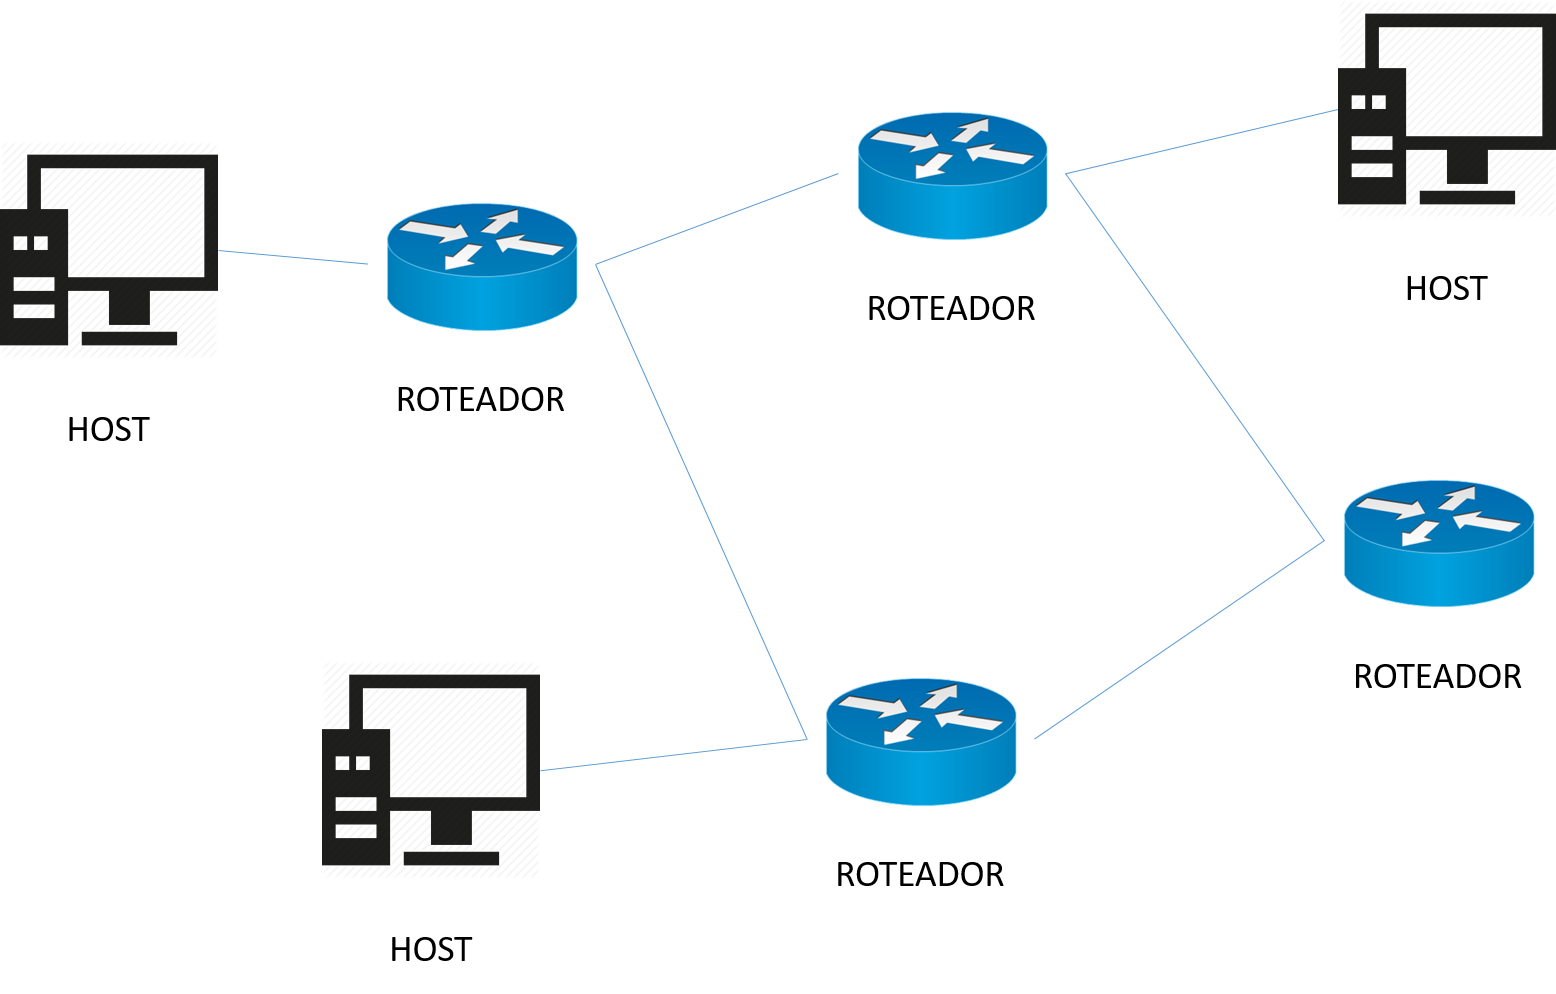
\includegraphics[width=0.7\textwidth]{Introducao/Rede.png}
\caption{Estrutura de uma Rede}
\label{Fig_Rede}
\end{figure}

Essa estrutura se mostrou extremamente eficiente, e permitiu que a expansão em nível mundial da Internet, uma vez que diversas redes com tamanhos e topologias diferentes conseguem se comunicar. 

Proporcional à expansão da Internet e a criação de cada vez mais dispositivos capazes de usá-la, houve um grande aumento no fluxo de dados. Tal aumento advém de práticas como o consumo de vídeo, através de plataformas como Youtube, Netflix, etc, sendo este o tipo de dado mais consumido e o segundo que mais cresce desde 2017\cite{CISCO}

Portanto, devido a essa progressiva demanda, novas arquiteturas de rede estão sendo investigadas. Contudo, como o núcleo da arquitetura atual, ou seja, os nós de comutação, são implementados via hardware, a implementação de arquiteturas experimentais se torna pouco viável, devido aos grandes custos dessa mudança de hardware, além do fato que essa troca iria interromper o fluxo de produção atual de uma rede, fator que dificulta o teste e validação de novas arquiteturas em ambientes reais, principalmente em redes de larga escala.

Dessa forma, soluções baseadas em software se tornaram mais atraentes devido a possibilidade de serem implementadas sem troca de hardware e sem interrupção da rede. Uma dessas alternativas que tem ganhado destaque é o paradigma SDN(Software Defined NetWork) juntamente com o protocolo OpenFlow. Uma rede SDN, utiliza de um dispositivo chamado controlador, que se conecta a todos os nós da rede, para configurá-los de acordo com o gerente da rede. O protocolo Openflow é um protocolo voltado para as redes SDN, que permite que o controlador se comunique com os comutatores.

A implementação de redes SDN ainda está numa fase experimental, e por isso, diversas pesquisas estão sendo desenvolvidas para verificar a performance desse tipo de rede. Uma das grandes vantagens de uma rede SDN é a possibilidade de separar o tráfego de dados em fluxos diferentes, além de poder alterar a tabela de encaminhamento dos comutatores para atingir um melhor desempenho da rede. 

Dessa forma, o objetivo desse trabalho é a criação de uma aplicação capaz de monitorar o fluxo de uma rede e identificar o consumo de dados de vídeos, provenientes de duas das principais plataformas de streaming : Youtube e NetFlix. Essa aplicação será integrada a um tipo de controlador chamado POX e testada através de software capaz de simular redes fisicas, chamado Mininet. Os conceitos de SDN , protocolo OpenFlow e controlador POX serão explicados de forma mais detalhada no capítulo 2.

\section{Objetivos}
\subsection{Objetivo geral}
Implementar e avaliar o desempenho de uma aplicação de monitoramento e classificação de fluxos de dados, utilizando uma rede SDN , junto com um controlador do tipo POX.

\subsection{Objetivos Específicos}

\begin{itemize}
\item Criar e configurar um ambiente de rede SDN, onde seja possível gerar e capturar todo o tráfego da rede. 
\item Implementar um módulo de monitoramento do tráfego da rede, para análise posterior.
\item Implementar o módulo de identificação e classificação do tipo de dados que trafega pela rede.
\item Implementar um módulo de detecção e tratamento de falhas na rede, para que a aplicação possa priorizar um determino tipo de fluxo.
\item Utilizar um banco da dados SQL, para armazenar todos os dados gerados pela aplicação
\end{itemize}3
\section{Estrutura do Trabalho}
Este trabalho será estruturado em 5 capítulos. No capítulo 2 serão explicados mais profundamente os conceitos de paradigma SDN, protoloco OpenFlow, controlador POX, além de das estruturas da arquitetura atual da Internet. Os módulos criados para a aplicação, suas funcionalidades, especificações, e ferramentas utilizadas serão apresentados no capitulo 3, assim como o ambiente em que o módulo foi testado.

O capítulo 4 será feita uma exposição e análise dos resultados obtidos. E por fim, no capítulo 5 serão expostas as conclusões, considerações finais e trabalhos futuros.




\documentclass[
	% -- opções da classe memoir --
	12pt,				% tamanho da fonte
	openright,			% capítulos começam em pág ímpar (insere página vazia caso preciso)
	twoside,			% para impressão em verso e anverso. Oposto a oneside
	a4paper,			% tamanho do papel. 
	% -- opções da classe abntex2 --
	%chapter=TITLE,		% títulos de capítulos convertidos em letras maiúsculas
	%section=TITLE,		% títulos de seções convertidos em letras maiúsculas
	%subsection=TITLE,	% títulos de subseções convertidos em letras maiúsculas
	%subsubsection=TITLE,% títulos de subsubseções convertidos em letras maiúsculas
	% -- opções do pacote babel --
	english,			% idioma adicional para hifenização
	french,				% idioma adicional para hifenização
	spanish,			% idioma adicional para hifenização
	brazil,				% o último idioma é o principal do documento
	]{abntex2}

\usepackage{cmap}			% Mapear caracteres especiais no PDF
\usepackage{lmodern}			% Usa a fonte Latin Modern			
\usepackage[T1]{fontenc}		% Selecao de codigos de fonte.
\usepackage[utf8]{inputenc}		% Codificacao do documento (conversão automática dos acentos)
\usepackage{lastpage}			% Usado pela Ficha catalográfica
\usepackage{indentfirst}		           % Indenta o primeiro parágrafo de cada seção.
\usepackage{color}				% Controle das cores
\usepackage{graphicx}			% Inclusão de gráficos
\usepackage{lipsum}			% para geração de dummy text

\usepackage[brazilian,hyperpageref]{backref}   % Paginas com as citações na bibl
\usepackage[alf]{abntex2cite}	                         % Citações padrão ABNT
% Configurações do pacote backref
% Usado sem a opção hyperpageref de backref
\renewcommand{\backrefpagesname}{Citado na(s) página(s):~}
% Texto padrão antes do número das páginas
\renewcommand{\backref}{}
% Define os textos da citação
\renewcommand*{\backrefalt}[4]{
	\ifcase #1 %
		Nenhuma citação no texto.%
	\or
		Citado na página #2.%
	\else
		Citado #1 vezes nas páginas #2.%
	\fi}%
% ---


% ---
% Informações de dados para CAPA e FOLHA DE ROSTO
% ---
\titulo{Modelo de Monografia de \\ Trabalho de Conclusão de Curso com \abnTeX}
\autor{<Nome Completo do Aluno>}
\local{Belo Horizonte}
\data{2013}
\orientador{Prof. <Nome Completo do Orientador>}
%\coorientador{Prof. }
\instituicao{%
  Universidade Federal de Minas Gerais -- UFMG
  \par
  Escola de Engenharia
  \par
  Curso de Graduação em Engenharia Elétrica}
\tipotrabalho{Trabalho de Conclusão de Curso}
% O preambulo deve conter o tipo do trabalho, o objetivo, o nome da instituição e a área de concentração 
\preambulo{Monografia apresentada durante o Seminário dos Trabalhos de Conclusão do Curso de Graduação em Engenharia Elétrica da UFMG, como parte dos requisitos necessários à obtenção do título de Engenheiro Eletricista.}
% alterando o aspecto da cor azul
\definecolor{blue}{RGB}{41,5,195}

% informações do PDF
\makeatletter
\hypersetup{
     	%pagebackref=true,
		pdftitle={\@title}, 
		pdfauthor={\@author},
    	pdfsubject={\imprimirpreambulo},
	    pdfcreator={LaTeX with abnTeX2},
		pdfkeywords={abnt}{latex}{abntex}{abntex2}{trabalho acadêmico}, 
		colorlinks=true,       	% false: boxed links; true: colored links
    	linkcolor=blue,          	           % color of internal links
    	citecolor=blue,        		% color of links to bibliography
    	filecolor=magenta,      		% color of file links
		urlcolor=blue,
		bookmarksdepth=4
}
\makeatother
% O tamanho do parágrafo é dado por:
\setlength{\parindent}{1.3cm}

% Controle do espaçamento entre um parágrafo e outro:
\setlength{\parskip}{0.2cm}  % tente também \onelineskip
\makeindex

% Início do documento
% ----
\begin{document}
% Retira espaço extra obsoleto entre as frases.
\frenchspacing 
%\imprimircapa
%\imprimirfolhaderosto

%\include{Inicio_Dedicatoria_resumo}

% ----------------------------------------------------------
% Capítulo 1 - Introdução
% ----------------------------------------------------------

\include{Introducao/main}
\include{Revisao/main}
\include{Metodologia/main}
% ----------------------------------------------------------
% Capítulo 2 - Revisão Bibliográfica
% ----------------------------------------------------------

% ----------------------------------------------------------
% Capítulo 3 - Metodologia
% ----------------------------------------------------------



% ----------------------------------------------------------
% Capítulo 4 - Resultados e Discussao
% ----------------------------------------------------------

% ----------------------------------------------------------
% Capítulo 5 - Conclusões
% ----------------------------------------------------------

% ---
% Finaliza a parte no bookmark do PDF, para que se inicie o bookmark na raiz
% ---
\bookmarksetup{startatroot}% 
% ---

% ----------------------------------------------------------
% ELEMENTOS PÓS-TEXTUAIS
% ----------------------------------------------------------
\postextual

% ----------------------------------------------------------
% Referências bibliográficas
% ----------------------------------------------------------
\bibliography{abntex2-modelo-references}

% ----------------------------------------------------------
% Apêndices
% ----------------------------------------------------------

% ---
% Inicia os apêndices
% ---
% \begin{apendicesenv}

% % Imprime uma página indicando o início dos apêndices
% \partapendices

% % ----------------------------------------------------------
% \chapter{Quisque libero justo}
% % ----------------------------------------------------------

% \lipsum[50-54]

% % ----------------------------------------------------------
% \chapter{Nullam elementum urna vel imperdiet sodales elit ipsum pharetra}
% % ----------------------------------------------------------
% \lipsum[55-59]

% \end{apendicesenv}
% % ---

% % ----------------------------------------------------------
% % Anexos
% % ----------------------------------------------------------

% % ---
% % Inicia os anexos
% % ---
% \begin{anexosenv}

% % Imprime uma página indicando o início dos anexos
% \partanexos
% % ---
% \chapter{Morbi ultrices rutrum lorem}
% % ---
% \lipsum[60]

% % ---
% \chapter{Cras non urna sed feugiat cum sociis natoque penatibus}
% % ---
% \lipsum[61-63]

% % ---
% \chapter{Fusce facilisis lacinia dui}
% % ---
% \lipsum[64-65]

% \end{anexosenv}

\end{document}

\documentclass[
	% -- opções da classe memoir --
	12pt,				% tamanho da fonte
	openright,			% capítulos começam em pág ímpar (insere página vazia caso preciso)
	twoside,			% para impressão em verso e anverso. Oposto a oneside
	a4paper,			% tamanho do papel. 
	% -- opções da classe abntex2 --
	%chapter=TITLE,		% títulos de capítulos convertidos em letras maiúsculas
	%section=TITLE,		% títulos de seções convertidos em letras maiúsculas
	%subsection=TITLE,	% títulos de subseções convertidos em letras maiúsculas
	%subsubsection=TITLE,% títulos de subsubseções convertidos em letras maiúsculas
	% -- opções do pacote babel --
	english,			% idioma adicional para hifenização
	french,				% idioma adicional para hifenização
	spanish,			% idioma adicional para hifenização
	brazil,				% o último idioma é o principal do documento
	]{abntex2}

\usepackage{cmap}			% Mapear caracteres especiais no PDF
\usepackage{lmodern}			% Usa a fonte Latin Modern			
\usepackage[T1]{fontenc}		% Selecao de codigos de fonte.
\usepackage[utf8]{inputenc}		% Codificacao do documento (conversão automática dos acentos)
\usepackage{lastpage}			% Usado pela Ficha catalográfica
\usepackage{indentfirst}		           % Indenta o primeiro parágrafo de cada seção.
\usepackage{color}				% Controle das cores
\usepackage{graphicx}			% Inclusão de gráficos
\usepackage{lipsum}			% para geração de dummy text

\usepackage[brazilian,hyperpageref]{backref}   % Paginas com as citações na bibl
\usepackage[alf]{abntex2cite}	                         % Citações padrão ABNT
% Configurações do pacote backref
% Usado sem a opção hyperpageref de backref
\renewcommand{\backrefpagesname}{Citado na(s) página(s):~}
% Texto padrão antes do número das páginas
\renewcommand{\backref}{}
% Define os textos da citação
\renewcommand*{\backrefalt}[4]{
	\ifcase #1 %
		Nenhuma citação no texto.%
	\or
		Citado na página #2.%
	\else
		Citado #1 vezes nas páginas #2.%
	\fi}%
% ---


% ---
% Informações de dados para CAPA e FOLHA DE ROSTO
% ---
\titulo{Modelo de Monografia de \\ Trabalho de Conclusão de Curso com \abnTeX}
\autor{<Nome Completo do Aluno>}
\local{Belo Horizonte}
\data{2013}
\orientador{Prof. <Nome Completo do Orientador>}
%\coorientador{Prof. }
\instituicao{%
  Universidade Federal de Minas Gerais -- UFMG
  \par
  Escola de Engenharia
  \par
  Curso de Graduação em Engenharia Elétrica}
\tipotrabalho{Trabalho de Conclusão de Curso}
% O preambulo deve conter o tipo do trabalho, o objetivo, o nome da instituição e a área de concentração 
\preambulo{Monografia apresentada durante o Seminário dos Trabalhos de Conclusão do Curso de Graduação em Engenharia Elétrica da UFMG, como parte dos requisitos necessários à obtenção do título de Engenheiro Eletricista.}
% alterando o aspecto da cor azul
\definecolor{blue}{RGB}{41,5,195}

% informações do PDF
\makeatletter
\hypersetup{
     	%pagebackref=true,
		pdftitle={\@title}, 
		pdfauthor={\@author},
    	pdfsubject={\imprimirpreambulo},
	    pdfcreator={LaTeX with abnTeX2},
		pdfkeywords={abnt}{latex}{abntex}{abntex2}{trabalho acadêmico}, 
		colorlinks=true,       	% false: boxed links; true: colored links
    	linkcolor=blue,          	           % color of internal links
    	citecolor=blue,        		% color of links to bibliography
    	filecolor=magenta,      		% color of file links
		urlcolor=blue,
		bookmarksdepth=4
}
\makeatother
% O tamanho do parágrafo é dado por:
\setlength{\parindent}{1.3cm}

% Controle do espaçamento entre um parágrafo e outro:
\setlength{\parskip}{0.2cm}  % tente também \onelineskip
\makeindex

% Início do documento
% ----
\begin{document}
% Retira espaço extra obsoleto entre as frases.
\frenchspacing 
%\imprimircapa
%\imprimirfolhaderosto

%\include{Inicio_Dedicatoria_resumo}

% ----------------------------------------------------------
% Capítulo 1 - Introdução
% ----------------------------------------------------------

\include{Introducao/main}
\include{Revisao/main}
\include{Metodologia/main}
% ----------------------------------------------------------
% Capítulo 2 - Revisão Bibliográfica
% ----------------------------------------------------------

% ----------------------------------------------------------
% Capítulo 3 - Metodologia
% ----------------------------------------------------------



% ----------------------------------------------------------
% Capítulo 4 - Resultados e Discussao
% ----------------------------------------------------------

% ----------------------------------------------------------
% Capítulo 5 - Conclusões
% ----------------------------------------------------------

% ---
% Finaliza a parte no bookmark do PDF, para que se inicie o bookmark na raiz
% ---
\bookmarksetup{startatroot}% 
% ---

% ----------------------------------------------------------
% ELEMENTOS PÓS-TEXTUAIS
% ----------------------------------------------------------
\postextual

% ----------------------------------------------------------
% Referências bibliográficas
% ----------------------------------------------------------
\bibliography{abntex2-modelo-references}

% ----------------------------------------------------------
% Apêndices
% ----------------------------------------------------------

% ---
% Inicia os apêndices
% ---
% \begin{apendicesenv}

% % Imprime uma página indicando o início dos apêndices
% \partapendices

% % ----------------------------------------------------------
% \chapter{Quisque libero justo}
% % ----------------------------------------------------------

% \lipsum[50-54]

% % ----------------------------------------------------------
% \chapter{Nullam elementum urna vel imperdiet sodales elit ipsum pharetra}
% % ----------------------------------------------------------
% \lipsum[55-59]

% \end{apendicesenv}
% % ---

% % ----------------------------------------------------------
% % Anexos
% % ----------------------------------------------------------

% % ---
% % Inicia os anexos
% % ---
% \begin{anexosenv}

% % Imprime uma página indicando o início dos anexos
% \partanexos
% % ---
% \chapter{Morbi ultrices rutrum lorem}
% % ---
% \lipsum[60]

% % ---
% \chapter{Cras non urna sed feugiat cum sociis natoque penatibus}
% % ---
% \lipsum[61-63]

% % ---
% \chapter{Fusce facilisis lacinia dui}
% % ---
% \lipsum[64-65]

% \end{anexosenv}

\end{document}
% ----------------------------------------------------------
% Capítulo 2 - Revisão Bibliográfica
% ----------------------------------------------------------

% ----------------------------------------------------------
% Capítulo 3 - Metodologia
% ----------------------------------------------------------



% ----------------------------------------------------------
% Capítulo 4 - Resultados e Discussao
% ----------------------------------------------------------

% ----------------------------------------------------------
% Capítulo 5 - Conclusões
% ----------------------------------------------------------

% ---
% Finaliza a parte no bookmark do PDF, para que se inicie o bookmark na raiz
% ---
\bookmarksetup{startatroot}% 
% ---

% ----------------------------------------------------------
% ELEMENTOS PÓS-TEXTUAIS
% ----------------------------------------------------------
\postextual

% ----------------------------------------------------------
% Referências bibliográficas
% ----------------------------------------------------------
\bibliography{abntex2-modelo-references}

% ----------------------------------------------------------
% Apêndices
% ----------------------------------------------------------

% ---
% Inicia os apêndices
% ---
% \begin{apendicesenv}

% % Imprime uma página indicando o início dos apêndices
% \partapendices

% % ----------------------------------------------------------
% \chapter{Quisque libero justo}
% % ----------------------------------------------------------

% \lipsum[50-54]

% % ----------------------------------------------------------
% \chapter{Nullam elementum urna vel imperdiet sodales elit ipsum pharetra}
% % ----------------------------------------------------------
% \lipsum[55-59]

% \end{apendicesenv}
% % ---

% % ----------------------------------------------------------
% % Anexos
% % ----------------------------------------------------------

% % ---
% % Inicia os anexos
% % ---
% \begin{anexosenv}

% % Imprime uma página indicando o início dos anexos
% \partanexos
% % ---
% \chapter{Morbi ultrices rutrum lorem}
% % ---
% \lipsum[60]

% % ---
% \chapter{Cras non urna sed feugiat cum sociis natoque penatibus}
% % ---
% \lipsum[61-63]

% % ---
% \chapter{Fusce facilisis lacinia dui}
% % ---
% \lipsum[64-65]

% \end{anexosenv}

\end{document}

\documentclass[
	% -- opções da classe memoir --
	12pt,				% tamanho da fonte
	openright,			% capítulos começam em pág ímpar (insere página vazia caso preciso)
	twoside,			% para impressão em verso e anverso. Oposto a oneside
	a4paper,			% tamanho do papel. 
	% -- opções da classe abntex2 --
	%chapter=TITLE,		% títulos de capítulos convertidos em letras maiúsculas
	%section=TITLE,		% títulos de seções convertidos em letras maiúsculas
	%subsection=TITLE,	% títulos de subseções convertidos em letras maiúsculas
	%subsubsection=TITLE,% títulos de subsubseções convertidos em letras maiúsculas
	% -- opções do pacote babel --
	english,			% idioma adicional para hifenização
	french,				% idioma adicional para hifenização
	spanish,			% idioma adicional para hifenização
	brazil,				% o último idioma é o principal do documento
	]{abntex2}

\usepackage{cmap}			% Mapear caracteres especiais no PDF
\usepackage{lmodern}			% Usa a fonte Latin Modern			
\usepackage[T1]{fontenc}		% Selecao de codigos de fonte.
\usepackage[utf8]{inputenc}		% Codificacao do documento (conversão automática dos acentos)
\usepackage{lastpage}			% Usado pela Ficha catalográfica
\usepackage{indentfirst}		           % Indenta o primeiro parágrafo de cada seção.
\usepackage{color}				% Controle das cores
\usepackage{graphicx}			% Inclusão de gráficos
\usepackage{lipsum}			% para geração de dummy text

\usepackage[brazilian,hyperpageref]{backref}   % Paginas com as citações na bibl
\usepackage[alf]{abntex2cite}	                         % Citações padrão ABNT
% Configurações do pacote backref
% Usado sem a opção hyperpageref de backref
\renewcommand{\backrefpagesname}{Citado na(s) página(s):~}
% Texto padrão antes do número das páginas
\renewcommand{\backref}{}
% Define os textos da citação
\renewcommand*{\backrefalt}[4]{
	\ifcase #1 %
		Nenhuma citação no texto.%
	\or
		Citado na página #2.%
	\else
		Citado #1 vezes nas páginas #2.%
	\fi}%
% ---


% ---
% Informações de dados para CAPA e FOLHA DE ROSTO
% ---
\titulo{Modelo de Monografia de \\ Trabalho de Conclusão de Curso com \abnTeX}
\autor{<Nome Completo do Aluno>}
\local{Belo Horizonte}
\data{2013}
\orientador{Prof. <Nome Completo do Orientador>}
%\coorientador{Prof. }
\instituicao{%
  Universidade Federal de Minas Gerais -- UFMG
  \par
  Escola de Engenharia
  \par
  Curso de Graduação em Engenharia Elétrica}
\tipotrabalho{Trabalho de Conclusão de Curso}
% O preambulo deve conter o tipo do trabalho, o objetivo, o nome da instituição e a área de concentração 
\preambulo{Monografia apresentada durante o Seminário dos Trabalhos de Conclusão do Curso de Graduação em Engenharia Elétrica da UFMG, como parte dos requisitos necessários à obtenção do título de Engenheiro Eletricista.}
% alterando o aspecto da cor azul
\definecolor{blue}{RGB}{41,5,195}

% informações do PDF
\makeatletter
\hypersetup{
     	%pagebackref=true,
		pdftitle={\@title}, 
		pdfauthor={\@author},
    	pdfsubject={\imprimirpreambulo},
	    pdfcreator={LaTeX with abnTeX2},
		pdfkeywords={abnt}{latex}{abntex}{abntex2}{trabalho acadêmico}, 
		colorlinks=true,       	% false: boxed links; true: colored links
    	linkcolor=blue,          	           % color of internal links
    	citecolor=blue,        		% color of links to bibliography
    	filecolor=magenta,      		% color of file links
		urlcolor=blue,
		bookmarksdepth=4
}
\makeatother
% O tamanho do parágrafo é dado por:
\setlength{\parindent}{1.3cm}

% Controle do espaçamento entre um parágrafo e outro:
\setlength{\parskip}{0.2cm}  % tente também \onelineskip
\makeindex

% Início do documento
% ----
\begin{document}
% Retira espaço extra obsoleto entre as frases.
\frenchspacing 
%\imprimircapa
%\imprimirfolhaderosto

%
\begin{dedicatoria}
   \vspace*{\fill}
   \centering
   \noindent
   \textit{ Este trabalho é dedicado às crianças adultas que,\\
   quando pequenas, sonharam em se tornar cientistas.} \vspace*{\fill}
\end{dedicatoria}
\begin{agradecimentos}
\end{agradecimentos}

\begin{epigrafe}
    \vspace*{\fill}
	\begin{flushright}
		\textit{``Não vos amoldeis às estruturas deste mundo, \\
		mas transformai-vos pela renovação da mente, \\
		a fim de distinguir qual é a vontade de Deus: \\
		o que é bom, o que Lhe é agradável, o que é perfeito.\\
		(Bíblia Sagrada, Romanos 12, 2)}
	\end{flushright}
\end{epigrafe}
% ---

% ---
% RESUMOS
% ---
% resumo em português
\setlength{\absparsep}{18pt} % ajusta o espaçamento dos parágrafos do resumo
\begin{resumo}

 objetivo, o método, os resultados e as conclusões do documento. A ordem e a extensão
 destes itens dependem do tipo de resumo (informativo ou indicativo) e do
 tratamento que cada item recebe no documento original. O resumo deve ser
 precedido da referência do documento, com exceção do resumo inserido no
 próprio documento. (\ldots) As palavras-chave devem figurar logo abaixo do
 resumo, antecedidas da expressão Palavras-chave:, separadas entre si por
 ponto e finalizadas também por ponto.

 \textbf{Palavras-chaves}: latex. abntex. editoração de texto.
\end{resumo}

% resumo em inglês
\begin{resumo}[Abstract]
 \begin{otherlanguage*}{english}
   This is the english abstract.

   \vspace{\onelineskip}
 
   \noindent 
   \textbf{Key-words}: latex. abntex. text editoration.
 \end{otherlanguage*}
\end{resumo}

% ---
% inserir lista de ilustrações
% ---
\pdfbookmark[0]{\listfigurename}{lof}
\listoffigures*
\cleardoublepage
% ---

% ---
% inserir lista de tabelas
% ---
\pdfbookmark[0]{\listtablename}{lot}
\listoftables*
\cleardoublepage
% ---

% ---
% inserir lista de abreviaturas e siglas
% ---
\begin{siglas}
  \item[Fig.] Area of the $i^{th}$ component
  \item[456] Isto é um número
  \item[123] Isto é outro número
%  \item[lauro cesar] este é o meu nome
\end{siglas}
% ---

% ---
% inserir lista de símbolos
% ---
\begin{simbolos}
  \item[$ \Gamma $] Letra grega Gama
  \item[$ \Lambda $] Lambda
  \item[$ \zeta $] Letra grega minúscula zeta
  \item[$ \in $] Pertence
\end{simbolos}
% ---

% ---
% inserir o sumario
% ---
\pdfbookmark[0]{\contentsname}{toc}
\tableofcontents*
\cleardoublepage
% ---

% ----------------------------------------------------------
% ELEMENTOS TEXTUAIS
% ----------------------------------------------------------
\textual

% ----------------------------------------------------------
% Capítulo 1 - Introdução
% ----------------------------------------------------------


\chapter{Introdução}
 
A atual arquitetura de rede da Internet é composta por: nós de comutação (roteadores e switches, responsáveis pelo encaminhamento de pacotes de dados) e os hosts (máquinas de origem e destino de pacotes de dados, como computadores de usuários, servidores, smartphones, etc). Os nós de comutação possuem uma tabela que os indica qual é o próximo nó que um pacote deve ser encaminhado , chamada de tabela de encaminhamento. Como um pacote pode passar por múltiplos nós até chegar ao seu destino, e como o fluxo de pacotes em cada nó é extremamente alto, toda a operação de consulta a tabela de encaminhamento e transmissão de dados é realizado via hardware. Como o exemplo (Figura \ref{Fig_Rede}) onde observa-se uma rede de Internet de maneira simplificada .

\begin{figure}[h]
\centering
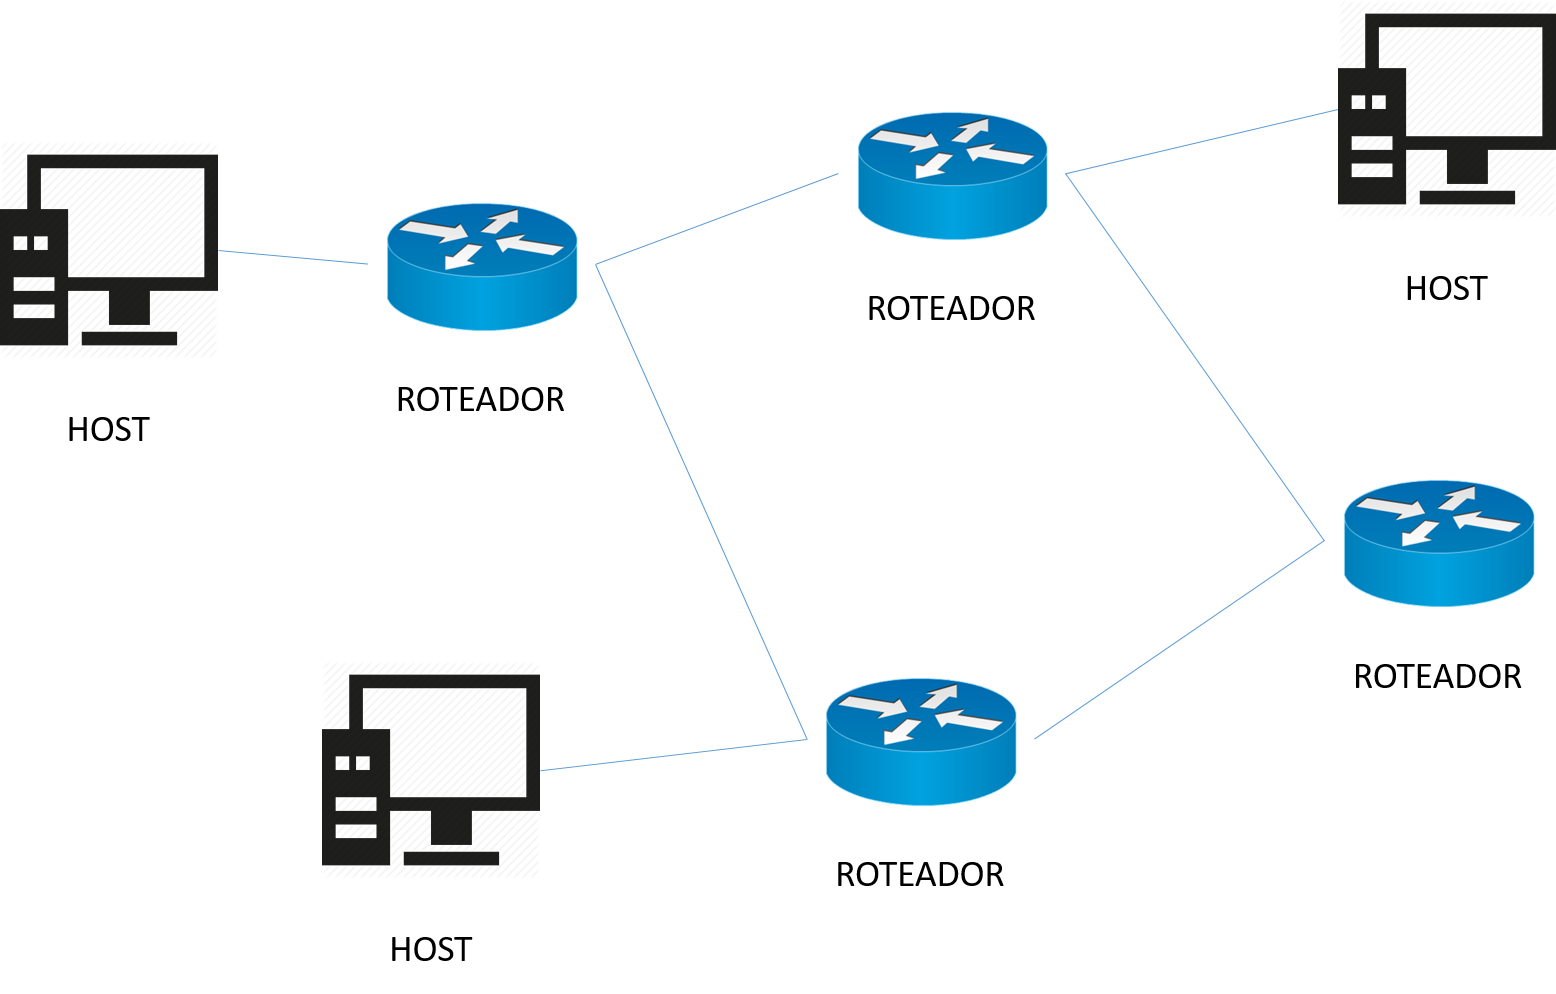
\includegraphics[width=0.7\textwidth]{Introducao/Rede.png}
\caption{Estrutura de uma Rede}
\label{Fig_Rede}
\end{figure}

Essa estrutura se mostrou extremamente eficiente, e permitiu que a expansão em nível mundial da Internet, uma vez que diversas redes com tamanhos e topologias diferentes conseguem se comunicar. 

Proporcional à expansão da Internet e a criação de cada vez mais dispositivos capazes de usá-la, houve um grande aumento no fluxo de dados. Tal aumento advém de práticas como o consumo de vídeo, através de plataformas como Youtube, Netflix, etc, sendo este o tipo de dado mais consumido e o segundo que mais cresce desde 2017\cite{CISCO}

Portanto, devido a essa progressiva demanda, novas arquiteturas de rede estão sendo investigadas. Contudo, como o núcleo da arquitetura atual, ou seja, os nós de comutação, são implementados via hardware, a implementação de arquiteturas experimentais se torna pouco viável, devido aos grandes custos dessa mudança de hardware, além do fato que essa troca iria interromper o fluxo de produção atual de uma rede, fator que dificulta o teste e validação de novas arquiteturas em ambientes reais, principalmente em redes de larga escala.

Dessa forma, soluções baseadas em software se tornaram mais atraentes devido a possibilidade de serem implementadas sem troca de hardware e sem interrupção da rede. Uma dessas alternativas que tem ganhado destaque é o paradigma SDN(Software Defined NetWork) juntamente com o protocolo OpenFlow. Uma rede SDN, utiliza de um dispositivo chamado controlador, que se conecta a todos os nós da rede, para configurá-los de acordo com o gerente da rede. O protocolo Openflow é um protocolo voltado para as redes SDN, que permite que o controlador se comunique com os comutatores.

A implementação de redes SDN ainda está numa fase experimental, e por isso, diversas pesquisas estão sendo desenvolvidas para verificar a performance desse tipo de rede. Uma das grandes vantagens de uma rede SDN é a possibilidade de separar o tráfego de dados em fluxos diferentes, além de poder alterar a tabela de encaminhamento dos comutatores para atingir um melhor desempenho da rede. 

Dessa forma, o objetivo desse trabalho é a criação de uma aplicação capaz de monitorar o fluxo de uma rede e identificar o consumo de dados de vídeos, provenientes de duas das principais plataformas de streaming : Youtube e NetFlix. Essa aplicação será integrada a um tipo de controlador chamado POX e testada através de software capaz de simular redes fisicas, chamado Mininet. Os conceitos de SDN , protocolo OpenFlow e controlador POX serão explicados de forma mais detalhada no capítulo 2.

\section{Objetivos}
\subsection{Objetivo geral}
Implementar e avaliar o desempenho de uma aplicação de monitoramento e classificação de fluxos de dados, utilizando uma rede SDN , junto com um controlador do tipo POX.

\subsection{Objetivos Específicos}

\begin{itemize}
\item Criar e configurar um ambiente de rede SDN, onde seja possível gerar e capturar todo o tráfego da rede. 
\item Implementar um módulo de monitoramento do tráfego da rede, para análise posterior.
\item Implementar o módulo de identificação e classificação do tipo de dados que trafega pela rede.
\item Implementar um módulo de detecção e tratamento de falhas na rede, para que a aplicação possa priorizar um determino tipo de fluxo.
\item Utilizar um banco da dados SQL, para armazenar todos os dados gerados pela aplicação
\end{itemize}3
\section{Estrutura do Trabalho}
Este trabalho será estruturado em 5 capítulos. No capítulo 2 serão explicados mais profundamente os conceitos de paradigma SDN, protoloco OpenFlow, controlador POX, além de das estruturas da arquitetura atual da Internet. Os módulos criados para a aplicação, suas funcionalidades, especificações, e ferramentas utilizadas serão apresentados no capitulo 3, assim como o ambiente em que o módulo foi testado.

O capítulo 4 será feita uma exposição e análise dos resultados obtidos. E por fim, no capítulo 5 serão expostas as conclusões, considerações finais e trabalhos futuros.




\documentclass[
	% -- opções da classe memoir --
	12pt,				% tamanho da fonte
	openright,			% capítulos começam em pág ímpar (insere página vazia caso preciso)
	twoside,			% para impressão em verso e anverso. Oposto a oneside
	a4paper,			% tamanho do papel. 
	% -- opções da classe abntex2 --
	%chapter=TITLE,		% títulos de capítulos convertidos em letras maiúsculas
	%section=TITLE,		% títulos de seções convertidos em letras maiúsculas
	%subsection=TITLE,	% títulos de subseções convertidos em letras maiúsculas
	%subsubsection=TITLE,% títulos de subsubseções convertidos em letras maiúsculas
	% -- opções do pacote babel --
	english,			% idioma adicional para hifenização
	french,				% idioma adicional para hifenização
	spanish,			% idioma adicional para hifenização
	brazil,				% o último idioma é o principal do documento
	]{abntex2}

\usepackage{cmap}			% Mapear caracteres especiais no PDF
\usepackage{lmodern}			% Usa a fonte Latin Modern			
\usepackage[T1]{fontenc}		% Selecao de codigos de fonte.
\usepackage[utf8]{inputenc}		% Codificacao do documento (conversão automática dos acentos)
\usepackage{lastpage}			% Usado pela Ficha catalográfica
\usepackage{indentfirst}		           % Indenta o primeiro parágrafo de cada seção.
\usepackage{color}				% Controle das cores
\usepackage{graphicx}			% Inclusão de gráficos
\usepackage{lipsum}			% para geração de dummy text

\usepackage[brazilian,hyperpageref]{backref}   % Paginas com as citações na bibl
\usepackage[alf]{abntex2cite}	                         % Citações padrão ABNT
% Configurações do pacote backref
% Usado sem a opção hyperpageref de backref
\renewcommand{\backrefpagesname}{Citado na(s) página(s):~}
% Texto padrão antes do número das páginas
\renewcommand{\backref}{}
% Define os textos da citação
\renewcommand*{\backrefalt}[4]{
	\ifcase #1 %
		Nenhuma citação no texto.%
	\or
		Citado na página #2.%
	\else
		Citado #1 vezes nas páginas #2.%
	\fi}%
% ---


% ---
% Informações de dados para CAPA e FOLHA DE ROSTO
% ---
\titulo{Modelo de Monografia de \\ Trabalho de Conclusão de Curso com \abnTeX}
\autor{<Nome Completo do Aluno>}
\local{Belo Horizonte}
\data{2013}
\orientador{Prof. <Nome Completo do Orientador>}
%\coorientador{Prof. }
\instituicao{%
  Universidade Federal de Minas Gerais -- UFMG
  \par
  Escola de Engenharia
  \par
  Curso de Graduação em Engenharia Elétrica}
\tipotrabalho{Trabalho de Conclusão de Curso}
% O preambulo deve conter o tipo do trabalho, o objetivo, o nome da instituição e a área de concentração 
\preambulo{Monografia apresentada durante o Seminário dos Trabalhos de Conclusão do Curso de Graduação em Engenharia Elétrica da UFMG, como parte dos requisitos necessários à obtenção do título de Engenheiro Eletricista.}
% alterando o aspecto da cor azul
\definecolor{blue}{RGB}{41,5,195}

% informações do PDF
\makeatletter
\hypersetup{
     	%pagebackref=true,
		pdftitle={\@title}, 
		pdfauthor={\@author},
    	pdfsubject={\imprimirpreambulo},
	    pdfcreator={LaTeX with abnTeX2},
		pdfkeywords={abnt}{latex}{abntex}{abntex2}{trabalho acadêmico}, 
		colorlinks=true,       	% false: boxed links; true: colored links
    	linkcolor=blue,          	           % color of internal links
    	citecolor=blue,        		% color of links to bibliography
    	filecolor=magenta,      		% color of file links
		urlcolor=blue,
		bookmarksdepth=4
}
\makeatother
% O tamanho do parágrafo é dado por:
\setlength{\parindent}{1.3cm}

% Controle do espaçamento entre um parágrafo e outro:
\setlength{\parskip}{0.2cm}  % tente também \onelineskip
\makeindex

% Início do documento
% ----
\begin{document}
% Retira espaço extra obsoleto entre as frases.
\frenchspacing 
%\imprimircapa
%\imprimirfolhaderosto

%\include{Inicio_Dedicatoria_resumo}

% ----------------------------------------------------------
% Capítulo 1 - Introdução
% ----------------------------------------------------------

\include{Introducao/main}
\include{Revisao/main}
\include{Metodologia/main}
% ----------------------------------------------------------
% Capítulo 2 - Revisão Bibliográfica
% ----------------------------------------------------------

% ----------------------------------------------------------
% Capítulo 3 - Metodologia
% ----------------------------------------------------------



% ----------------------------------------------------------
% Capítulo 4 - Resultados e Discussao
% ----------------------------------------------------------

% ----------------------------------------------------------
% Capítulo 5 - Conclusões
% ----------------------------------------------------------

% ---
% Finaliza a parte no bookmark do PDF, para que se inicie o bookmark na raiz
% ---
\bookmarksetup{startatroot}% 
% ---

% ----------------------------------------------------------
% ELEMENTOS PÓS-TEXTUAIS
% ----------------------------------------------------------
\postextual

% ----------------------------------------------------------
% Referências bibliográficas
% ----------------------------------------------------------
\bibliography{abntex2-modelo-references}

% ----------------------------------------------------------
% Apêndices
% ----------------------------------------------------------

% ---
% Inicia os apêndices
% ---
% \begin{apendicesenv}

% % Imprime uma página indicando o início dos apêndices
% \partapendices

% % ----------------------------------------------------------
% \chapter{Quisque libero justo}
% % ----------------------------------------------------------

% \lipsum[50-54]

% % ----------------------------------------------------------
% \chapter{Nullam elementum urna vel imperdiet sodales elit ipsum pharetra}
% % ----------------------------------------------------------
% \lipsum[55-59]

% \end{apendicesenv}
% % ---

% % ----------------------------------------------------------
% % Anexos
% % ----------------------------------------------------------

% % ---
% % Inicia os anexos
% % ---
% \begin{anexosenv}

% % Imprime uma página indicando o início dos anexos
% \partanexos
% % ---
% \chapter{Morbi ultrices rutrum lorem}
% % ---
% \lipsum[60]

% % ---
% \chapter{Cras non urna sed feugiat cum sociis natoque penatibus}
% % ---
% \lipsum[61-63]

% % ---
% \chapter{Fusce facilisis lacinia dui}
% % ---
% \lipsum[64-65]

% \end{anexosenv}

\end{document}

\documentclass[
	% -- opções da classe memoir --
	12pt,				% tamanho da fonte
	openright,			% capítulos começam em pág ímpar (insere página vazia caso preciso)
	twoside,			% para impressão em verso e anverso. Oposto a oneside
	a4paper,			% tamanho do papel. 
	% -- opções da classe abntex2 --
	%chapter=TITLE,		% títulos de capítulos convertidos em letras maiúsculas
	%section=TITLE,		% títulos de seções convertidos em letras maiúsculas
	%subsection=TITLE,	% títulos de subseções convertidos em letras maiúsculas
	%subsubsection=TITLE,% títulos de subsubseções convertidos em letras maiúsculas
	% -- opções do pacote babel --
	english,			% idioma adicional para hifenização
	french,				% idioma adicional para hifenização
	spanish,			% idioma adicional para hifenização
	brazil,				% o último idioma é o principal do documento
	]{abntex2}

\usepackage{cmap}			% Mapear caracteres especiais no PDF
\usepackage{lmodern}			% Usa a fonte Latin Modern			
\usepackage[T1]{fontenc}		% Selecao de codigos de fonte.
\usepackage[utf8]{inputenc}		% Codificacao do documento (conversão automática dos acentos)
\usepackage{lastpage}			% Usado pela Ficha catalográfica
\usepackage{indentfirst}		           % Indenta o primeiro parágrafo de cada seção.
\usepackage{color}				% Controle das cores
\usepackage{graphicx}			% Inclusão de gráficos
\usepackage{lipsum}			% para geração de dummy text

\usepackage[brazilian,hyperpageref]{backref}   % Paginas com as citações na bibl
\usepackage[alf]{abntex2cite}	                         % Citações padrão ABNT
% Configurações do pacote backref
% Usado sem a opção hyperpageref de backref
\renewcommand{\backrefpagesname}{Citado na(s) página(s):~}
% Texto padrão antes do número das páginas
\renewcommand{\backref}{}
% Define os textos da citação
\renewcommand*{\backrefalt}[4]{
	\ifcase #1 %
		Nenhuma citação no texto.%
	\or
		Citado na página #2.%
	\else
		Citado #1 vezes nas páginas #2.%
	\fi}%
% ---


% ---
% Informações de dados para CAPA e FOLHA DE ROSTO
% ---
\titulo{Modelo de Monografia de \\ Trabalho de Conclusão de Curso com \abnTeX}
\autor{<Nome Completo do Aluno>}
\local{Belo Horizonte}
\data{2013}
\orientador{Prof. <Nome Completo do Orientador>}
%\coorientador{Prof. }
\instituicao{%
  Universidade Federal de Minas Gerais -- UFMG
  \par
  Escola de Engenharia
  \par
  Curso de Graduação em Engenharia Elétrica}
\tipotrabalho{Trabalho de Conclusão de Curso}
% O preambulo deve conter o tipo do trabalho, o objetivo, o nome da instituição e a área de concentração 
\preambulo{Monografia apresentada durante o Seminário dos Trabalhos de Conclusão do Curso de Graduação em Engenharia Elétrica da UFMG, como parte dos requisitos necessários à obtenção do título de Engenheiro Eletricista.}
% alterando o aspecto da cor azul
\definecolor{blue}{RGB}{41,5,195}

% informações do PDF
\makeatletter
\hypersetup{
     	%pagebackref=true,
		pdftitle={\@title}, 
		pdfauthor={\@author},
    	pdfsubject={\imprimirpreambulo},
	    pdfcreator={LaTeX with abnTeX2},
		pdfkeywords={abnt}{latex}{abntex}{abntex2}{trabalho acadêmico}, 
		colorlinks=true,       	% false: boxed links; true: colored links
    	linkcolor=blue,          	           % color of internal links
    	citecolor=blue,        		% color of links to bibliography
    	filecolor=magenta,      		% color of file links
		urlcolor=blue,
		bookmarksdepth=4
}
\makeatother
% O tamanho do parágrafo é dado por:
\setlength{\parindent}{1.3cm}

% Controle do espaçamento entre um parágrafo e outro:
\setlength{\parskip}{0.2cm}  % tente também \onelineskip
\makeindex

% Início do documento
% ----
\begin{document}
% Retira espaço extra obsoleto entre as frases.
\frenchspacing 
%\imprimircapa
%\imprimirfolhaderosto

%\include{Inicio_Dedicatoria_resumo}

% ----------------------------------------------------------
% Capítulo 1 - Introdução
% ----------------------------------------------------------

\include{Introducao/main}
\include{Revisao/main}
\include{Metodologia/main}
% ----------------------------------------------------------
% Capítulo 2 - Revisão Bibliográfica
% ----------------------------------------------------------

% ----------------------------------------------------------
% Capítulo 3 - Metodologia
% ----------------------------------------------------------



% ----------------------------------------------------------
% Capítulo 4 - Resultados e Discussao
% ----------------------------------------------------------

% ----------------------------------------------------------
% Capítulo 5 - Conclusões
% ----------------------------------------------------------

% ---
% Finaliza a parte no bookmark do PDF, para que se inicie o bookmark na raiz
% ---
\bookmarksetup{startatroot}% 
% ---

% ----------------------------------------------------------
% ELEMENTOS PÓS-TEXTUAIS
% ----------------------------------------------------------
\postextual

% ----------------------------------------------------------
% Referências bibliográficas
% ----------------------------------------------------------
\bibliography{abntex2-modelo-references}

% ----------------------------------------------------------
% Apêndices
% ----------------------------------------------------------

% ---
% Inicia os apêndices
% ---
% \begin{apendicesenv}

% % Imprime uma página indicando o início dos apêndices
% \partapendices

% % ----------------------------------------------------------
% \chapter{Quisque libero justo}
% % ----------------------------------------------------------

% \lipsum[50-54]

% % ----------------------------------------------------------
% \chapter{Nullam elementum urna vel imperdiet sodales elit ipsum pharetra}
% % ----------------------------------------------------------
% \lipsum[55-59]

% \end{apendicesenv}
% % ---

% % ----------------------------------------------------------
% % Anexos
% % ----------------------------------------------------------

% % ---
% % Inicia os anexos
% % ---
% \begin{anexosenv}

% % Imprime uma página indicando o início dos anexos
% \partanexos
% % ---
% \chapter{Morbi ultrices rutrum lorem}
% % ---
% \lipsum[60]

% % ---
% \chapter{Cras non urna sed feugiat cum sociis natoque penatibus}
% % ---
% \lipsum[61-63]

% % ---
% \chapter{Fusce facilisis lacinia dui}
% % ---
% \lipsum[64-65]

% \end{anexosenv}

\end{document}
% ----------------------------------------------------------
% Capítulo 2 - Revisão Bibliográfica
% ----------------------------------------------------------

% ----------------------------------------------------------
% Capítulo 3 - Metodologia
% ----------------------------------------------------------



% ----------------------------------------------------------
% Capítulo 4 - Resultados e Discussao
% ----------------------------------------------------------

% ----------------------------------------------------------
% Capítulo 5 - Conclusões
% ----------------------------------------------------------

% ---
% Finaliza a parte no bookmark do PDF, para que se inicie o bookmark na raiz
% ---
\bookmarksetup{startatroot}% 
% ---

% ----------------------------------------------------------
% ELEMENTOS PÓS-TEXTUAIS
% ----------------------------------------------------------
\postextual

% ----------------------------------------------------------
% Referências bibliográficas
% ----------------------------------------------------------
\bibliography{abntex2-modelo-references}

% ----------------------------------------------------------
% Apêndices
% ----------------------------------------------------------

% ---
% Inicia os apêndices
% ---
% \begin{apendicesenv}

% % Imprime uma página indicando o início dos apêndices
% \partapendices

% % ----------------------------------------------------------
% \chapter{Quisque libero justo}
% % ----------------------------------------------------------

% \lipsum[50-54]

% % ----------------------------------------------------------
% \chapter{Nullam elementum urna vel imperdiet sodales elit ipsum pharetra}
% % ----------------------------------------------------------
% \lipsum[55-59]

% \end{apendicesenv}
% % ---

% % ----------------------------------------------------------
% % Anexos
% % ----------------------------------------------------------

% % ---
% % Inicia os anexos
% % ---
% \begin{anexosenv}

% % Imprime uma página indicando o início dos anexos
% \partanexos
% % ---
% \chapter{Morbi ultrices rutrum lorem}
% % ---
% \lipsum[60]

% % ---
% \chapter{Cras non urna sed feugiat cum sociis natoque penatibus}
% % ---
% \lipsum[61-63]

% % ---
% \chapter{Fusce facilisis lacinia dui}
% % ---
% \lipsum[64-65]

% \end{anexosenv}

\end{document}
% ----------------------------------------------------------
% Capítulo 2 - Revisão Bibliográfica
% ----------------------------------------------------------

% ----------------------------------------------------------
% Capítulo 3 - Metodologia
% ----------------------------------------------------------



% ----------------------------------------------------------
% Capítulo 4 - Resultados e Discussao
% ----------------------------------------------------------

% ----------------------------------------------------------
% Capítulo 5 - Conclusões
% ----------------------------------------------------------

% ---
% Finaliza a parte no bookmark do PDF, para que se inicie o bookmark na raiz
% ---
\bookmarksetup{startatroot}% 
% ---

% ----------------------------------------------------------
% ELEMENTOS PÓS-TEXTUAIS
% ----------------------------------------------------------
\postextual

% ----------------------------------------------------------
% Referências bibliográficas
% ----------------------------------------------------------
\bibliography{abntex2-modelo-references}

% ----------------------------------------------------------
% Apêndices
% ----------------------------------------------------------

% ---
% Inicia os apêndices
% ---
% \begin{apendicesenv}

% % Imprime uma página indicando o início dos apêndices
% \partapendices

% % ----------------------------------------------------------
% \chapter{Quisque libero justo}
% % ----------------------------------------------------------

% \lipsum[50-54]

% % ----------------------------------------------------------
% \chapter{Nullam elementum urna vel imperdiet sodales elit ipsum pharetra}
% % ----------------------------------------------------------
% \lipsum[55-59]

% \end{apendicesenv}
% % ---

% % ----------------------------------------------------------
% % Anexos
% % ----------------------------------------------------------

% % ---
% % Inicia os anexos
% % ---
% \begin{anexosenv}

% % Imprime uma página indicando o início dos anexos
% \partanexos
% % ---
% \chapter{Morbi ultrices rutrum lorem}
% % ---
% \lipsum[60]

% % ---
% \chapter{Cras non urna sed feugiat cum sociis natoque penatibus}
% % ---
% \lipsum[61-63]

% % ---
% \chapter{Fusce facilisis lacinia dui}
% % ---
% \lipsum[64-65]

% \end{anexosenv}

\end{document}

\documentclass[
	% -- opções da classe memoir --
	12pt,				% tamanho da fonte
	openright,			% capítulos começam em pág ímpar (insere página vazia caso preciso)
	twoside,			% para impressão em verso e anverso. Oposto a oneside
	a4paper,			% tamanho do papel. 
	% -- opções da classe abntex2 --
	%chapter=TITLE,		% títulos de capítulos convertidos em letras maiúsculas
	%section=TITLE,		% títulos de seções convertidos em letras maiúsculas
	%subsection=TITLE,	% títulos de subseções convertidos em letras maiúsculas
	%subsubsection=TITLE,% títulos de subsubseções convertidos em letras maiúsculas
	% -- opções do pacote babel --
	english,			% idioma adicional para hifenização
	french,				% idioma adicional para hifenização
	spanish,			% idioma adicional para hifenização
	brazil,				% o último idioma é o principal do documento
	]{abntex2}

\usepackage{cmap}			% Mapear caracteres especiais no PDF
\usepackage{lmodern}			% Usa a fonte Latin Modern			
\usepackage[T1]{fontenc}		% Selecao de codigos de fonte.
\usepackage[utf8]{inputenc}		% Codificacao do documento (conversão automática dos acentos)
\usepackage{lastpage}			% Usado pela Ficha catalográfica
\usepackage{indentfirst}		           % Indenta o primeiro parágrafo de cada seção.
\usepackage{color}				% Controle das cores
\usepackage{graphicx}			% Inclusão de gráficos
\usepackage{lipsum}			% para geração de dummy text

\usepackage[brazilian,hyperpageref]{backref}   % Paginas com as citações na bibl
\usepackage[alf]{abntex2cite}	                         % Citações padrão ABNT
% Configurações do pacote backref
% Usado sem a opção hyperpageref de backref
\renewcommand{\backrefpagesname}{Citado na(s) página(s):~}
% Texto padrão antes do número das páginas
\renewcommand{\backref}{}
% Define os textos da citação
\renewcommand*{\backrefalt}[4]{
	\ifcase #1 %
		Nenhuma citação no texto.%
	\or
		Citado na página #2.%
	\else
		Citado #1 vezes nas páginas #2.%
	\fi}%
% ---


% ---
% Informações de dados para CAPA e FOLHA DE ROSTO
% ---
\titulo{Modelo de Monografia de \\ Trabalho de Conclusão de Curso com \abnTeX}
\autor{<Nome Completo do Aluno>}
\local{Belo Horizonte}
\data{2013}
\orientador{Prof. <Nome Completo do Orientador>}
%\coorientador{Prof. }
\instituicao{%
  Universidade Federal de Minas Gerais -- UFMG
  \par
  Escola de Engenharia
  \par
  Curso de Graduação em Engenharia Elétrica}
\tipotrabalho{Trabalho de Conclusão de Curso}
% O preambulo deve conter o tipo do trabalho, o objetivo, o nome da instituição e a área de concentração 
\preambulo{Monografia apresentada durante o Seminário dos Trabalhos de Conclusão do Curso de Graduação em Engenharia Elétrica da UFMG, como parte dos requisitos necessários à obtenção do título de Engenheiro Eletricista.}
% alterando o aspecto da cor azul
\definecolor{blue}{RGB}{41,5,195}

% informações do PDF
\makeatletter
\hypersetup{
     	%pagebackref=true,
		pdftitle={\@title}, 
		pdfauthor={\@author},
    	pdfsubject={\imprimirpreambulo},
	    pdfcreator={LaTeX with abnTeX2},
		pdfkeywords={abnt}{latex}{abntex}{abntex2}{trabalho acadêmico}, 
		colorlinks=true,       	% false: boxed links; true: colored links
    	linkcolor=blue,          	           % color of internal links
    	citecolor=blue,        		% color of links to bibliography
    	filecolor=magenta,      		% color of file links
		urlcolor=blue,
		bookmarksdepth=4
}
\makeatother
% O tamanho do parágrafo é dado por:
\setlength{\parindent}{1.3cm}

% Controle do espaçamento entre um parágrafo e outro:
\setlength{\parskip}{0.2cm}  % tente também \onelineskip
\makeindex

% Início do documento
% ----
\begin{document}
% Retira espaço extra obsoleto entre as frases.
\frenchspacing 
%\imprimircapa
%\imprimirfolhaderosto

%
\begin{dedicatoria}
   \vspace*{\fill}
   \centering
   \noindent
   \textit{ Este trabalho é dedicado às crianças adultas que,\\
   quando pequenas, sonharam em se tornar cientistas.} \vspace*{\fill}
\end{dedicatoria}
\begin{agradecimentos}
\end{agradecimentos}

\begin{epigrafe}
    \vspace*{\fill}
	\begin{flushright}
		\textit{``Não vos amoldeis às estruturas deste mundo, \\
		mas transformai-vos pela renovação da mente, \\
		a fim de distinguir qual é a vontade de Deus: \\
		o que é bom, o que Lhe é agradável, o que é perfeito.\\
		(Bíblia Sagrada, Romanos 12, 2)}
	\end{flushright}
\end{epigrafe}
% ---

% ---
% RESUMOS
% ---
% resumo em português
\setlength{\absparsep}{18pt} % ajusta o espaçamento dos parágrafos do resumo
\begin{resumo}

 objetivo, o método, os resultados e as conclusões do documento. A ordem e a extensão
 destes itens dependem do tipo de resumo (informativo ou indicativo) e do
 tratamento que cada item recebe no documento original. O resumo deve ser
 precedido da referência do documento, com exceção do resumo inserido no
 próprio documento. (\ldots) As palavras-chave devem figurar logo abaixo do
 resumo, antecedidas da expressão Palavras-chave:, separadas entre si por
 ponto e finalizadas também por ponto.

 \textbf{Palavras-chaves}: latex. abntex. editoração de texto.
\end{resumo}

% resumo em inglês
\begin{resumo}[Abstract]
 \begin{otherlanguage*}{english}
   This is the english abstract.

   \vspace{\onelineskip}
 
   \noindent 
   \textbf{Key-words}: latex. abntex. text editoration.
 \end{otherlanguage*}
\end{resumo}

% ---
% inserir lista de ilustrações
% ---
\pdfbookmark[0]{\listfigurename}{lof}
\listoffigures*
\cleardoublepage
% ---

% ---
% inserir lista de tabelas
% ---
\pdfbookmark[0]{\listtablename}{lot}
\listoftables*
\cleardoublepage
% ---

% ---
% inserir lista de abreviaturas e siglas
% ---
\begin{siglas}
  \item[Fig.] Area of the $i^{th}$ component
  \item[456] Isto é um número
  \item[123] Isto é outro número
%  \item[lauro cesar] este é o meu nome
\end{siglas}
% ---

% ---
% inserir lista de símbolos
% ---
\begin{simbolos}
  \item[$ \Gamma $] Letra grega Gama
  \item[$ \Lambda $] Lambda
  \item[$ \zeta $] Letra grega minúscula zeta
  \item[$ \in $] Pertence
\end{simbolos}
% ---

% ---
% inserir o sumario
% ---
\pdfbookmark[0]{\contentsname}{toc}
\tableofcontents*
\cleardoublepage
% ---

% ----------------------------------------------------------
% ELEMENTOS TEXTUAIS
% ----------------------------------------------------------
\textual

% ----------------------------------------------------------
% Capítulo 1 - Introdução
% ----------------------------------------------------------


\chapter{Introdução}
 
A atual arquitetura de rede da Internet é composta por: nós de comutação (roteadores e switches, responsáveis pelo encaminhamento de pacotes de dados) e os hosts (máquinas de origem e destino de pacotes de dados, como computadores de usuários, servidores, smartphones, etc). Os nós de comutação possuem uma tabela que os indica qual é o próximo nó que um pacote deve ser encaminhado , chamada de tabela de encaminhamento. Como um pacote pode passar por múltiplos nós até chegar ao seu destino, e como o fluxo de pacotes em cada nó é extremamente alto, toda a operação de consulta a tabela de encaminhamento e transmissão de dados é realizado via hardware. Como o exemplo (Figura \ref{Fig_Rede}) onde observa-se uma rede de Internet de maneira simplificada .

\begin{figure}[h]
\centering
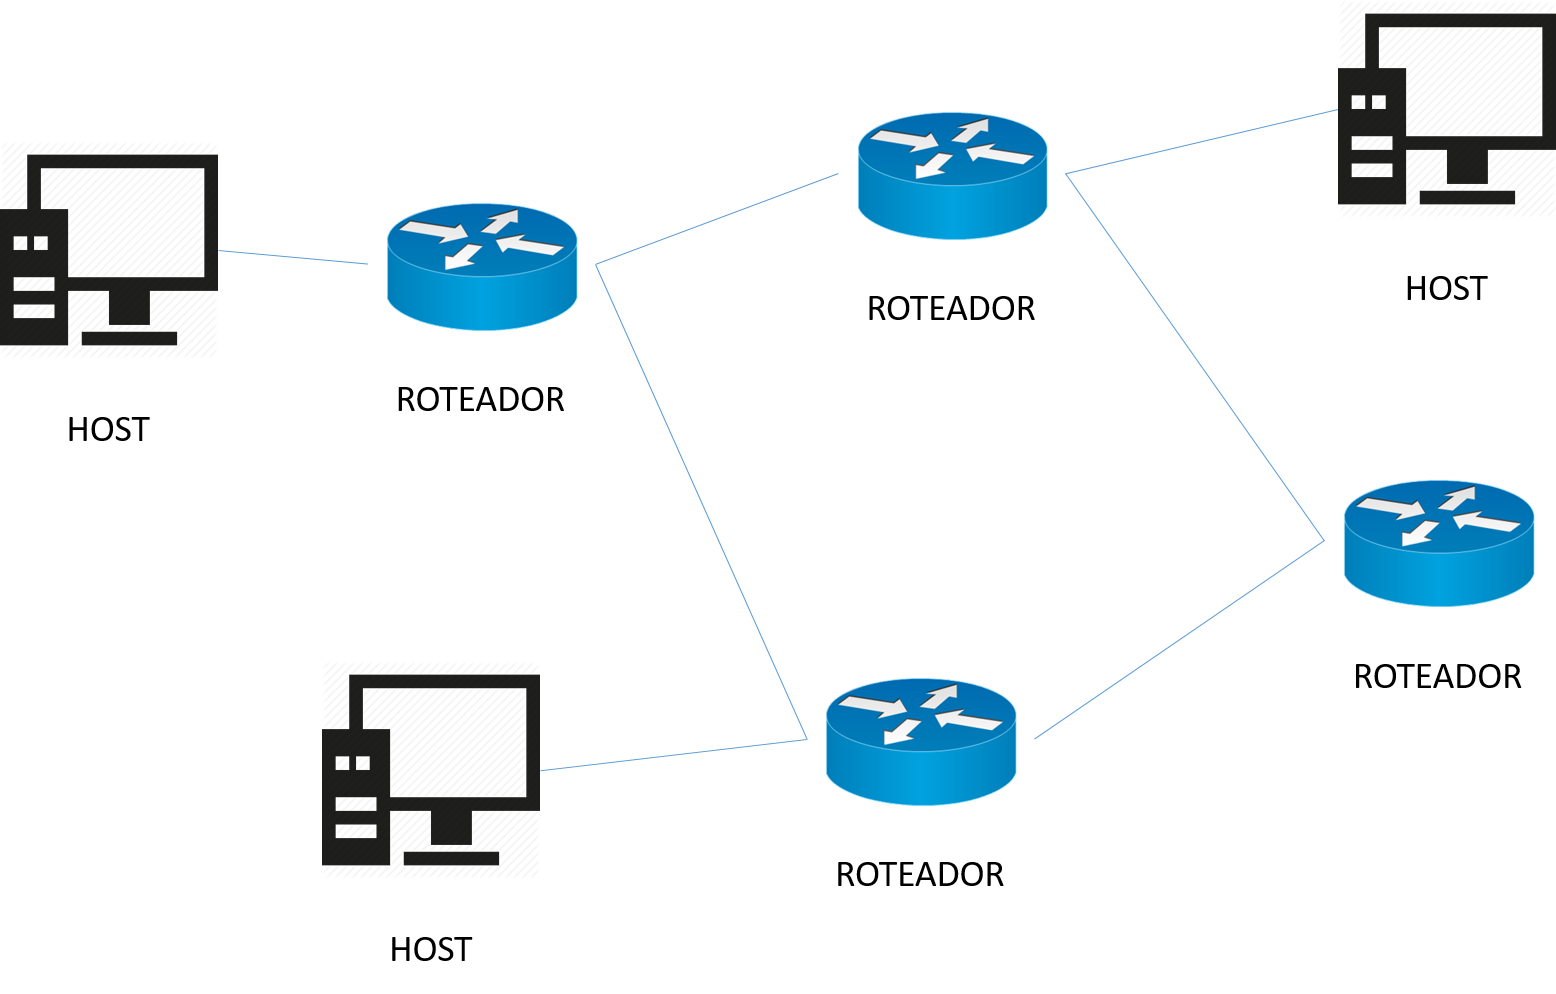
\includegraphics[width=0.7\textwidth]{Introducao/Rede.png}
\caption{Estrutura de uma Rede}
\label{Fig_Rede}
\end{figure}

Essa estrutura se mostrou extremamente eficiente, e permitiu que a expansão em nível mundial da Internet, uma vez que diversas redes com tamanhos e topologias diferentes conseguem se comunicar. 

Proporcional à expansão da Internet e a criação de cada vez mais dispositivos capazes de usá-la, houve um grande aumento no fluxo de dados. Tal aumento advém de práticas como o consumo de vídeo, através de plataformas como Youtube, Netflix, etc, sendo este o tipo de dado mais consumido e o segundo que mais cresce desde 2017\cite{CISCO}

Portanto, devido a essa progressiva demanda, novas arquiteturas de rede estão sendo investigadas. Contudo, como o núcleo da arquitetura atual, ou seja, os nós de comutação, são implementados via hardware, a implementação de arquiteturas experimentais se torna pouco viável, devido aos grandes custos dessa mudança de hardware, além do fato que essa troca iria interromper o fluxo de produção atual de uma rede, fator que dificulta o teste e validação de novas arquiteturas em ambientes reais, principalmente em redes de larga escala.

Dessa forma, soluções baseadas em software se tornaram mais atraentes devido a possibilidade de serem implementadas sem troca de hardware e sem interrupção da rede. Uma dessas alternativas que tem ganhado destaque é o paradigma SDN(Software Defined NetWork) juntamente com o protocolo OpenFlow. Uma rede SDN, utiliza de um dispositivo chamado controlador, que se conecta a todos os nós da rede, para configurá-los de acordo com o gerente da rede. O protocolo Openflow é um protocolo voltado para as redes SDN, que permite que o controlador se comunique com os comutatores.

A implementação de redes SDN ainda está numa fase experimental, e por isso, diversas pesquisas estão sendo desenvolvidas para verificar a performance desse tipo de rede. Uma das grandes vantagens de uma rede SDN é a possibilidade de separar o tráfego de dados em fluxos diferentes, além de poder alterar a tabela de encaminhamento dos comutatores para atingir um melhor desempenho da rede. 

Dessa forma, o objetivo desse trabalho é a criação de uma aplicação capaz de monitorar o fluxo de uma rede e identificar o consumo de dados de vídeos, provenientes de duas das principais plataformas de streaming : Youtube e NetFlix. Essa aplicação será integrada a um tipo de controlador chamado POX e testada através de software capaz de simular redes fisicas, chamado Mininet. Os conceitos de SDN , protocolo OpenFlow e controlador POX serão explicados de forma mais detalhada no capítulo 2.

\section{Objetivos}
\subsection{Objetivo geral}
Implementar e avaliar o desempenho de uma aplicação de monitoramento e classificação de fluxos de dados, utilizando uma rede SDN , junto com um controlador do tipo POX.

\subsection{Objetivos Específicos}

\begin{itemize}
\item Criar e configurar um ambiente de rede SDN, onde seja possível gerar e capturar todo o tráfego da rede. 
\item Implementar um módulo de monitoramento do tráfego da rede, para análise posterior.
\item Implementar o módulo de identificação e classificação do tipo de dados que trafega pela rede.
\item Implementar um módulo de detecção e tratamento de falhas na rede, para que a aplicação possa priorizar um determino tipo de fluxo.
\item Utilizar um banco da dados SQL, para armazenar todos os dados gerados pela aplicação
\end{itemize}3
\section{Estrutura do Trabalho}
Este trabalho será estruturado em 5 capítulos. No capítulo 2 serão explicados mais profundamente os conceitos de paradigma SDN, protoloco OpenFlow, controlador POX, além de das estruturas da arquitetura atual da Internet. Os módulos criados para a aplicação, suas funcionalidades, especificações, e ferramentas utilizadas serão apresentados no capitulo 3, assim como o ambiente em que o módulo foi testado.

O capítulo 4 será feita uma exposição e análise dos resultados obtidos. E por fim, no capítulo 5 serão expostas as conclusões, considerações finais e trabalhos futuros.




\documentclass[
	% -- opções da classe memoir --
	12pt,				% tamanho da fonte
	openright,			% capítulos começam em pág ímpar (insere página vazia caso preciso)
	twoside,			% para impressão em verso e anverso. Oposto a oneside
	a4paper,			% tamanho do papel. 
	% -- opções da classe abntex2 --
	%chapter=TITLE,		% títulos de capítulos convertidos em letras maiúsculas
	%section=TITLE,		% títulos de seções convertidos em letras maiúsculas
	%subsection=TITLE,	% títulos de subseções convertidos em letras maiúsculas
	%subsubsection=TITLE,% títulos de subsubseções convertidos em letras maiúsculas
	% -- opções do pacote babel --
	english,			% idioma adicional para hifenização
	french,				% idioma adicional para hifenização
	spanish,			% idioma adicional para hifenização
	brazil,				% o último idioma é o principal do documento
	]{abntex2}

\usepackage{cmap}			% Mapear caracteres especiais no PDF
\usepackage{lmodern}			% Usa a fonte Latin Modern			
\usepackage[T1]{fontenc}		% Selecao de codigos de fonte.
\usepackage[utf8]{inputenc}		% Codificacao do documento (conversão automática dos acentos)
\usepackage{lastpage}			% Usado pela Ficha catalográfica
\usepackage{indentfirst}		           % Indenta o primeiro parágrafo de cada seção.
\usepackage{color}				% Controle das cores
\usepackage{graphicx}			% Inclusão de gráficos
\usepackage{lipsum}			% para geração de dummy text

\usepackage[brazilian,hyperpageref]{backref}   % Paginas com as citações na bibl
\usepackage[alf]{abntex2cite}	                         % Citações padrão ABNT
% Configurações do pacote backref
% Usado sem a opção hyperpageref de backref
\renewcommand{\backrefpagesname}{Citado na(s) página(s):~}
% Texto padrão antes do número das páginas
\renewcommand{\backref}{}
% Define os textos da citação
\renewcommand*{\backrefalt}[4]{
	\ifcase #1 %
		Nenhuma citação no texto.%
	\or
		Citado na página #2.%
	\else
		Citado #1 vezes nas páginas #2.%
	\fi}%
% ---


% ---
% Informações de dados para CAPA e FOLHA DE ROSTO
% ---
\titulo{Modelo de Monografia de \\ Trabalho de Conclusão de Curso com \abnTeX}
\autor{<Nome Completo do Aluno>}
\local{Belo Horizonte}
\data{2013}
\orientador{Prof. <Nome Completo do Orientador>}
%\coorientador{Prof. }
\instituicao{%
  Universidade Federal de Minas Gerais -- UFMG
  \par
  Escola de Engenharia
  \par
  Curso de Graduação em Engenharia Elétrica}
\tipotrabalho{Trabalho de Conclusão de Curso}
% O preambulo deve conter o tipo do trabalho, o objetivo, o nome da instituição e a área de concentração 
\preambulo{Monografia apresentada durante o Seminário dos Trabalhos de Conclusão do Curso de Graduação em Engenharia Elétrica da UFMG, como parte dos requisitos necessários à obtenção do título de Engenheiro Eletricista.}
% alterando o aspecto da cor azul
\definecolor{blue}{RGB}{41,5,195}

% informações do PDF
\makeatletter
\hypersetup{
     	%pagebackref=true,
		pdftitle={\@title}, 
		pdfauthor={\@author},
    	pdfsubject={\imprimirpreambulo},
	    pdfcreator={LaTeX with abnTeX2},
		pdfkeywords={abnt}{latex}{abntex}{abntex2}{trabalho acadêmico}, 
		colorlinks=true,       	% false: boxed links; true: colored links
    	linkcolor=blue,          	           % color of internal links
    	citecolor=blue,        		% color of links to bibliography
    	filecolor=magenta,      		% color of file links
		urlcolor=blue,
		bookmarksdepth=4
}
\makeatother
% O tamanho do parágrafo é dado por:
\setlength{\parindent}{1.3cm}

% Controle do espaçamento entre um parágrafo e outro:
\setlength{\parskip}{0.2cm}  % tente também \onelineskip
\makeindex

% Início do documento
% ----
\begin{document}
% Retira espaço extra obsoleto entre as frases.
\frenchspacing 
%\imprimircapa
%\imprimirfolhaderosto

%
\begin{dedicatoria}
   \vspace*{\fill}
   \centering
   \noindent
   \textit{ Este trabalho é dedicado às crianças adultas que,\\
   quando pequenas, sonharam em se tornar cientistas.} \vspace*{\fill}
\end{dedicatoria}
\begin{agradecimentos}
\end{agradecimentos}

\begin{epigrafe}
    \vspace*{\fill}
	\begin{flushright}
		\textit{``Não vos amoldeis às estruturas deste mundo, \\
		mas transformai-vos pela renovação da mente, \\
		a fim de distinguir qual é a vontade de Deus: \\
		o que é bom, o que Lhe é agradável, o que é perfeito.\\
		(Bíblia Sagrada, Romanos 12, 2)}
	\end{flushright}
\end{epigrafe}
% ---

% ---
% RESUMOS
% ---
% resumo em português
\setlength{\absparsep}{18pt} % ajusta o espaçamento dos parágrafos do resumo
\begin{resumo}

 objetivo, o método, os resultados e as conclusões do documento. A ordem e a extensão
 destes itens dependem do tipo de resumo (informativo ou indicativo) e do
 tratamento que cada item recebe no documento original. O resumo deve ser
 precedido da referência do documento, com exceção do resumo inserido no
 próprio documento. (\ldots) As palavras-chave devem figurar logo abaixo do
 resumo, antecedidas da expressão Palavras-chave:, separadas entre si por
 ponto e finalizadas também por ponto.

 \textbf{Palavras-chaves}: latex. abntex. editoração de texto.
\end{resumo}

% resumo em inglês
\begin{resumo}[Abstract]
 \begin{otherlanguage*}{english}
   This is the english abstract.

   \vspace{\onelineskip}
 
   \noindent 
   \textbf{Key-words}: latex. abntex. text editoration.
 \end{otherlanguage*}
\end{resumo}

% ---
% inserir lista de ilustrações
% ---
\pdfbookmark[0]{\listfigurename}{lof}
\listoffigures*
\cleardoublepage
% ---

% ---
% inserir lista de tabelas
% ---
\pdfbookmark[0]{\listtablename}{lot}
\listoftables*
\cleardoublepage
% ---

% ---
% inserir lista de abreviaturas e siglas
% ---
\begin{siglas}
  \item[Fig.] Area of the $i^{th}$ component
  \item[456] Isto é um número
  \item[123] Isto é outro número
%  \item[lauro cesar] este é o meu nome
\end{siglas}
% ---

% ---
% inserir lista de símbolos
% ---
\begin{simbolos}
  \item[$ \Gamma $] Letra grega Gama
  \item[$ \Lambda $] Lambda
  \item[$ \zeta $] Letra grega minúscula zeta
  \item[$ \in $] Pertence
\end{simbolos}
% ---

% ---
% inserir o sumario
% ---
\pdfbookmark[0]{\contentsname}{toc}
\tableofcontents*
\cleardoublepage
% ---

% ----------------------------------------------------------
% ELEMENTOS TEXTUAIS
% ----------------------------------------------------------
\textual

% ----------------------------------------------------------
% Capítulo 1 - Introdução
% ----------------------------------------------------------


\chapter{Introdução}
 
A atual arquitetura de rede da Internet é composta por: nós de comutação (roteadores e switches, responsáveis pelo encaminhamento de pacotes de dados) e os hosts (máquinas de origem e destino de pacotes de dados, como computadores de usuários, servidores, smartphones, etc). Os nós de comutação possuem uma tabela que os indica qual é o próximo nó que um pacote deve ser encaminhado , chamada de tabela de encaminhamento. Como um pacote pode passar por múltiplos nós até chegar ao seu destino, e como o fluxo de pacotes em cada nó é extremamente alto, toda a operação de consulta a tabela de encaminhamento e transmissão de dados é realizado via hardware. Como o exemplo (Figura \ref{Fig_Rede}) onde observa-se uma rede de Internet de maneira simplificada .

\begin{figure}[h]
\centering
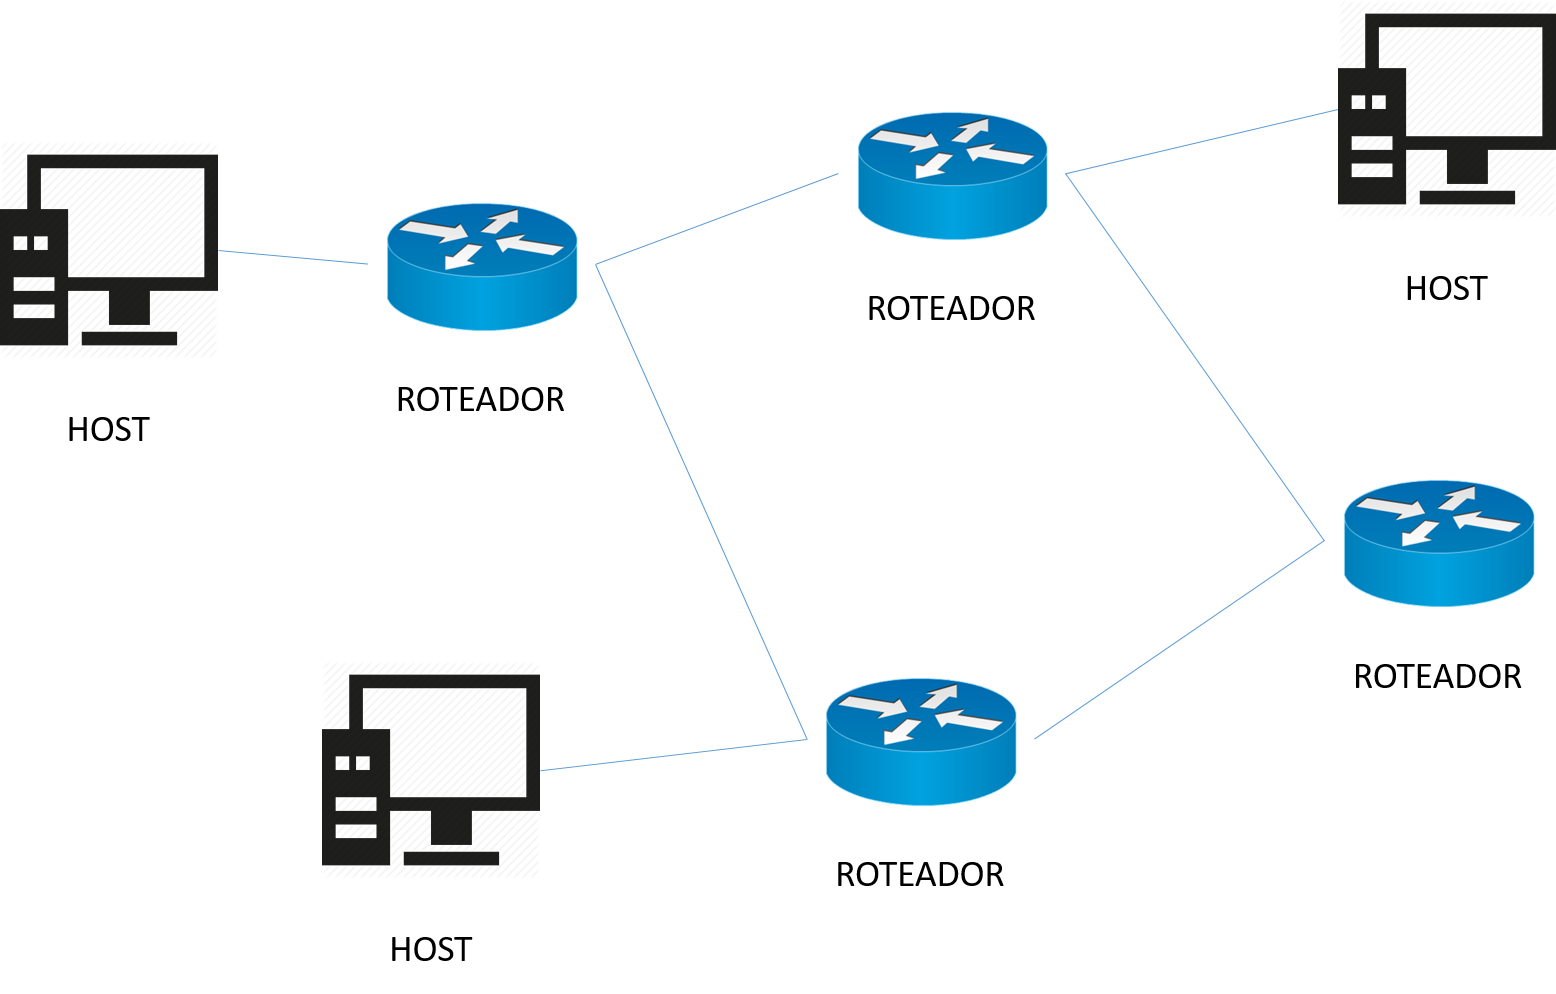
\includegraphics[width=0.7\textwidth]{Introducao/Rede.png}
\caption{Estrutura de uma Rede}
\label{Fig_Rede}
\end{figure}

Essa estrutura se mostrou extremamente eficiente, e permitiu que a expansão em nível mundial da Internet, uma vez que diversas redes com tamanhos e topologias diferentes conseguem se comunicar. 

Proporcional à expansão da Internet e a criação de cada vez mais dispositivos capazes de usá-la, houve um grande aumento no fluxo de dados. Tal aumento advém de práticas como o consumo de vídeo, através de plataformas como Youtube, Netflix, etc, sendo este o tipo de dado mais consumido e o segundo que mais cresce desde 2017\cite{CISCO}

Portanto, devido a essa progressiva demanda, novas arquiteturas de rede estão sendo investigadas. Contudo, como o núcleo da arquitetura atual, ou seja, os nós de comutação, são implementados via hardware, a implementação de arquiteturas experimentais se torna pouco viável, devido aos grandes custos dessa mudança de hardware, além do fato que essa troca iria interromper o fluxo de produção atual de uma rede, fator que dificulta o teste e validação de novas arquiteturas em ambientes reais, principalmente em redes de larga escala.

Dessa forma, soluções baseadas em software se tornaram mais atraentes devido a possibilidade de serem implementadas sem troca de hardware e sem interrupção da rede. Uma dessas alternativas que tem ganhado destaque é o paradigma SDN(Software Defined NetWork) juntamente com o protocolo OpenFlow. Uma rede SDN, utiliza de um dispositivo chamado controlador, que se conecta a todos os nós da rede, para configurá-los de acordo com o gerente da rede. O protocolo Openflow é um protocolo voltado para as redes SDN, que permite que o controlador se comunique com os comutatores.

A implementação de redes SDN ainda está numa fase experimental, e por isso, diversas pesquisas estão sendo desenvolvidas para verificar a performance desse tipo de rede. Uma das grandes vantagens de uma rede SDN é a possibilidade de separar o tráfego de dados em fluxos diferentes, além de poder alterar a tabela de encaminhamento dos comutatores para atingir um melhor desempenho da rede. 

Dessa forma, o objetivo desse trabalho é a criação de uma aplicação capaz de monitorar o fluxo de uma rede e identificar o consumo de dados de vídeos, provenientes de duas das principais plataformas de streaming : Youtube e NetFlix. Essa aplicação será integrada a um tipo de controlador chamado POX e testada através de software capaz de simular redes fisicas, chamado Mininet. Os conceitos de SDN , protocolo OpenFlow e controlador POX serão explicados de forma mais detalhada no capítulo 2.

\section{Objetivos}
\subsection{Objetivo geral}
Implementar e avaliar o desempenho de uma aplicação de monitoramento e classificação de fluxos de dados, utilizando uma rede SDN , junto com um controlador do tipo POX.

\subsection{Objetivos Específicos}

\begin{itemize}
\item Criar e configurar um ambiente de rede SDN, onde seja possível gerar e capturar todo o tráfego da rede. 
\item Implementar um módulo de monitoramento do tráfego da rede, para análise posterior.
\item Implementar o módulo de identificação e classificação do tipo de dados que trafega pela rede.
\item Implementar um módulo de detecção e tratamento de falhas na rede, para que a aplicação possa priorizar um determino tipo de fluxo.
\item Utilizar um banco da dados SQL, para armazenar todos os dados gerados pela aplicação
\end{itemize}3
\section{Estrutura do Trabalho}
Este trabalho será estruturado em 5 capítulos. No capítulo 2 serão explicados mais profundamente os conceitos de paradigma SDN, protoloco OpenFlow, controlador POX, além de das estruturas da arquitetura atual da Internet. Os módulos criados para a aplicação, suas funcionalidades, especificações, e ferramentas utilizadas serão apresentados no capitulo 3, assim como o ambiente em que o módulo foi testado.

O capítulo 4 será feita uma exposição e análise dos resultados obtidos. E por fim, no capítulo 5 serão expostas as conclusões, considerações finais e trabalhos futuros.




\documentclass[
	% -- opções da classe memoir --
	12pt,				% tamanho da fonte
	openright,			% capítulos começam em pág ímpar (insere página vazia caso preciso)
	twoside,			% para impressão em verso e anverso. Oposto a oneside
	a4paper,			% tamanho do papel. 
	% -- opções da classe abntex2 --
	%chapter=TITLE,		% títulos de capítulos convertidos em letras maiúsculas
	%section=TITLE,		% títulos de seções convertidos em letras maiúsculas
	%subsection=TITLE,	% títulos de subseções convertidos em letras maiúsculas
	%subsubsection=TITLE,% títulos de subsubseções convertidos em letras maiúsculas
	% -- opções do pacote babel --
	english,			% idioma adicional para hifenização
	french,				% idioma adicional para hifenização
	spanish,			% idioma adicional para hifenização
	brazil,				% o último idioma é o principal do documento
	]{abntex2}

\usepackage{cmap}			% Mapear caracteres especiais no PDF
\usepackage{lmodern}			% Usa a fonte Latin Modern			
\usepackage[T1]{fontenc}		% Selecao de codigos de fonte.
\usepackage[utf8]{inputenc}		% Codificacao do documento (conversão automática dos acentos)
\usepackage{lastpage}			% Usado pela Ficha catalográfica
\usepackage{indentfirst}		           % Indenta o primeiro parágrafo de cada seção.
\usepackage{color}				% Controle das cores
\usepackage{graphicx}			% Inclusão de gráficos
\usepackage{lipsum}			% para geração de dummy text

\usepackage[brazilian,hyperpageref]{backref}   % Paginas com as citações na bibl
\usepackage[alf]{abntex2cite}	                         % Citações padrão ABNT
% Configurações do pacote backref
% Usado sem a opção hyperpageref de backref
\renewcommand{\backrefpagesname}{Citado na(s) página(s):~}
% Texto padrão antes do número das páginas
\renewcommand{\backref}{}
% Define os textos da citação
\renewcommand*{\backrefalt}[4]{
	\ifcase #1 %
		Nenhuma citação no texto.%
	\or
		Citado na página #2.%
	\else
		Citado #1 vezes nas páginas #2.%
	\fi}%
% ---


% ---
% Informações de dados para CAPA e FOLHA DE ROSTO
% ---
\titulo{Modelo de Monografia de \\ Trabalho de Conclusão de Curso com \abnTeX}
\autor{<Nome Completo do Aluno>}
\local{Belo Horizonte}
\data{2013}
\orientador{Prof. <Nome Completo do Orientador>}
%\coorientador{Prof. }
\instituicao{%
  Universidade Federal de Minas Gerais -- UFMG
  \par
  Escola de Engenharia
  \par
  Curso de Graduação em Engenharia Elétrica}
\tipotrabalho{Trabalho de Conclusão de Curso}
% O preambulo deve conter o tipo do trabalho, o objetivo, o nome da instituição e a área de concentração 
\preambulo{Monografia apresentada durante o Seminário dos Trabalhos de Conclusão do Curso de Graduação em Engenharia Elétrica da UFMG, como parte dos requisitos necessários à obtenção do título de Engenheiro Eletricista.}
% alterando o aspecto da cor azul
\definecolor{blue}{RGB}{41,5,195}

% informações do PDF
\makeatletter
\hypersetup{
     	%pagebackref=true,
		pdftitle={\@title}, 
		pdfauthor={\@author},
    	pdfsubject={\imprimirpreambulo},
	    pdfcreator={LaTeX with abnTeX2},
		pdfkeywords={abnt}{latex}{abntex}{abntex2}{trabalho acadêmico}, 
		colorlinks=true,       	% false: boxed links; true: colored links
    	linkcolor=blue,          	           % color of internal links
    	citecolor=blue,        		% color of links to bibliography
    	filecolor=magenta,      		% color of file links
		urlcolor=blue,
		bookmarksdepth=4
}
\makeatother
% O tamanho do parágrafo é dado por:
\setlength{\parindent}{1.3cm}

% Controle do espaçamento entre um parágrafo e outro:
\setlength{\parskip}{0.2cm}  % tente também \onelineskip
\makeindex

% Início do documento
% ----
\begin{document}
% Retira espaço extra obsoleto entre as frases.
\frenchspacing 
%\imprimircapa
%\imprimirfolhaderosto

%\include{Inicio_Dedicatoria_resumo}

% ----------------------------------------------------------
% Capítulo 1 - Introdução
% ----------------------------------------------------------

\include{Introducao/main}
\include{Revisao/main}
\include{Metodologia/main}
% ----------------------------------------------------------
% Capítulo 2 - Revisão Bibliográfica
% ----------------------------------------------------------

% ----------------------------------------------------------
% Capítulo 3 - Metodologia
% ----------------------------------------------------------



% ----------------------------------------------------------
% Capítulo 4 - Resultados e Discussao
% ----------------------------------------------------------

% ----------------------------------------------------------
% Capítulo 5 - Conclusões
% ----------------------------------------------------------

% ---
% Finaliza a parte no bookmark do PDF, para que se inicie o bookmark na raiz
% ---
\bookmarksetup{startatroot}% 
% ---

% ----------------------------------------------------------
% ELEMENTOS PÓS-TEXTUAIS
% ----------------------------------------------------------
\postextual

% ----------------------------------------------------------
% Referências bibliográficas
% ----------------------------------------------------------
\bibliography{abntex2-modelo-references}

% ----------------------------------------------------------
% Apêndices
% ----------------------------------------------------------

% ---
% Inicia os apêndices
% ---
% \begin{apendicesenv}

% % Imprime uma página indicando o início dos apêndices
% \partapendices

% % ----------------------------------------------------------
% \chapter{Quisque libero justo}
% % ----------------------------------------------------------

% \lipsum[50-54]

% % ----------------------------------------------------------
% \chapter{Nullam elementum urna vel imperdiet sodales elit ipsum pharetra}
% % ----------------------------------------------------------
% \lipsum[55-59]

% \end{apendicesenv}
% % ---

% % ----------------------------------------------------------
% % Anexos
% % ----------------------------------------------------------

% % ---
% % Inicia os anexos
% % ---
% \begin{anexosenv}

% % Imprime uma página indicando o início dos anexos
% \partanexos
% % ---
% \chapter{Morbi ultrices rutrum lorem}
% % ---
% \lipsum[60]

% % ---
% \chapter{Cras non urna sed feugiat cum sociis natoque penatibus}
% % ---
% \lipsum[61-63]

% % ---
% \chapter{Fusce facilisis lacinia dui}
% % ---
% \lipsum[64-65]

% \end{anexosenv}

\end{document}

\documentclass[
	% -- opções da classe memoir --
	12pt,				% tamanho da fonte
	openright,			% capítulos começam em pág ímpar (insere página vazia caso preciso)
	twoside,			% para impressão em verso e anverso. Oposto a oneside
	a4paper,			% tamanho do papel. 
	% -- opções da classe abntex2 --
	%chapter=TITLE,		% títulos de capítulos convertidos em letras maiúsculas
	%section=TITLE,		% títulos de seções convertidos em letras maiúsculas
	%subsection=TITLE,	% títulos de subseções convertidos em letras maiúsculas
	%subsubsection=TITLE,% títulos de subsubseções convertidos em letras maiúsculas
	% -- opções do pacote babel --
	english,			% idioma adicional para hifenização
	french,				% idioma adicional para hifenização
	spanish,			% idioma adicional para hifenização
	brazil,				% o último idioma é o principal do documento
	]{abntex2}

\usepackage{cmap}			% Mapear caracteres especiais no PDF
\usepackage{lmodern}			% Usa a fonte Latin Modern			
\usepackage[T1]{fontenc}		% Selecao de codigos de fonte.
\usepackage[utf8]{inputenc}		% Codificacao do documento (conversão automática dos acentos)
\usepackage{lastpage}			% Usado pela Ficha catalográfica
\usepackage{indentfirst}		           % Indenta o primeiro parágrafo de cada seção.
\usepackage{color}				% Controle das cores
\usepackage{graphicx}			% Inclusão de gráficos
\usepackage{lipsum}			% para geração de dummy text

\usepackage[brazilian,hyperpageref]{backref}   % Paginas com as citações na bibl
\usepackage[alf]{abntex2cite}	                         % Citações padrão ABNT
% Configurações do pacote backref
% Usado sem a opção hyperpageref de backref
\renewcommand{\backrefpagesname}{Citado na(s) página(s):~}
% Texto padrão antes do número das páginas
\renewcommand{\backref}{}
% Define os textos da citação
\renewcommand*{\backrefalt}[4]{
	\ifcase #1 %
		Nenhuma citação no texto.%
	\or
		Citado na página #2.%
	\else
		Citado #1 vezes nas páginas #2.%
	\fi}%
% ---


% ---
% Informações de dados para CAPA e FOLHA DE ROSTO
% ---
\titulo{Modelo de Monografia de \\ Trabalho de Conclusão de Curso com \abnTeX}
\autor{<Nome Completo do Aluno>}
\local{Belo Horizonte}
\data{2013}
\orientador{Prof. <Nome Completo do Orientador>}
%\coorientador{Prof. }
\instituicao{%
  Universidade Federal de Minas Gerais -- UFMG
  \par
  Escola de Engenharia
  \par
  Curso de Graduação em Engenharia Elétrica}
\tipotrabalho{Trabalho de Conclusão de Curso}
% O preambulo deve conter o tipo do trabalho, o objetivo, o nome da instituição e a área de concentração 
\preambulo{Monografia apresentada durante o Seminário dos Trabalhos de Conclusão do Curso de Graduação em Engenharia Elétrica da UFMG, como parte dos requisitos necessários à obtenção do título de Engenheiro Eletricista.}
% alterando o aspecto da cor azul
\definecolor{blue}{RGB}{41,5,195}

% informações do PDF
\makeatletter
\hypersetup{
     	%pagebackref=true,
		pdftitle={\@title}, 
		pdfauthor={\@author},
    	pdfsubject={\imprimirpreambulo},
	    pdfcreator={LaTeX with abnTeX2},
		pdfkeywords={abnt}{latex}{abntex}{abntex2}{trabalho acadêmico}, 
		colorlinks=true,       	% false: boxed links; true: colored links
    	linkcolor=blue,          	           % color of internal links
    	citecolor=blue,        		% color of links to bibliography
    	filecolor=magenta,      		% color of file links
		urlcolor=blue,
		bookmarksdepth=4
}
\makeatother
% O tamanho do parágrafo é dado por:
\setlength{\parindent}{1.3cm}

% Controle do espaçamento entre um parágrafo e outro:
\setlength{\parskip}{0.2cm}  % tente também \onelineskip
\makeindex

% Início do documento
% ----
\begin{document}
% Retira espaço extra obsoleto entre as frases.
\frenchspacing 
%\imprimircapa
%\imprimirfolhaderosto

%\include{Inicio_Dedicatoria_resumo}

% ----------------------------------------------------------
% Capítulo 1 - Introdução
% ----------------------------------------------------------

\include{Introducao/main}
\include{Revisao/main}
\include{Metodologia/main}
% ----------------------------------------------------------
% Capítulo 2 - Revisão Bibliográfica
% ----------------------------------------------------------

% ----------------------------------------------------------
% Capítulo 3 - Metodologia
% ----------------------------------------------------------



% ----------------------------------------------------------
% Capítulo 4 - Resultados e Discussao
% ----------------------------------------------------------

% ----------------------------------------------------------
% Capítulo 5 - Conclusões
% ----------------------------------------------------------

% ---
% Finaliza a parte no bookmark do PDF, para que se inicie o bookmark na raiz
% ---
\bookmarksetup{startatroot}% 
% ---

% ----------------------------------------------------------
% ELEMENTOS PÓS-TEXTUAIS
% ----------------------------------------------------------
\postextual

% ----------------------------------------------------------
% Referências bibliográficas
% ----------------------------------------------------------
\bibliography{abntex2-modelo-references}

% ----------------------------------------------------------
% Apêndices
% ----------------------------------------------------------

% ---
% Inicia os apêndices
% ---
% \begin{apendicesenv}

% % Imprime uma página indicando o início dos apêndices
% \partapendices

% % ----------------------------------------------------------
% \chapter{Quisque libero justo}
% % ----------------------------------------------------------

% \lipsum[50-54]

% % ----------------------------------------------------------
% \chapter{Nullam elementum urna vel imperdiet sodales elit ipsum pharetra}
% % ----------------------------------------------------------
% \lipsum[55-59]

% \end{apendicesenv}
% % ---

% % ----------------------------------------------------------
% % Anexos
% % ----------------------------------------------------------

% % ---
% % Inicia os anexos
% % ---
% \begin{anexosenv}

% % Imprime uma página indicando o início dos anexos
% \partanexos
% % ---
% \chapter{Morbi ultrices rutrum lorem}
% % ---
% \lipsum[60]

% % ---
% \chapter{Cras non urna sed feugiat cum sociis natoque penatibus}
% % ---
% \lipsum[61-63]

% % ---
% \chapter{Fusce facilisis lacinia dui}
% % ---
% \lipsum[64-65]

% \end{anexosenv}

\end{document}
% ----------------------------------------------------------
% Capítulo 2 - Revisão Bibliográfica
% ----------------------------------------------------------

% ----------------------------------------------------------
% Capítulo 3 - Metodologia
% ----------------------------------------------------------



% ----------------------------------------------------------
% Capítulo 4 - Resultados e Discussao
% ----------------------------------------------------------

% ----------------------------------------------------------
% Capítulo 5 - Conclusões
% ----------------------------------------------------------

% ---
% Finaliza a parte no bookmark do PDF, para que se inicie o bookmark na raiz
% ---
\bookmarksetup{startatroot}% 
% ---

% ----------------------------------------------------------
% ELEMENTOS PÓS-TEXTUAIS
% ----------------------------------------------------------
\postextual

% ----------------------------------------------------------
% Referências bibliográficas
% ----------------------------------------------------------
\bibliography{abntex2-modelo-references}

% ----------------------------------------------------------
% Apêndices
% ----------------------------------------------------------

% ---
% Inicia os apêndices
% ---
% \begin{apendicesenv}

% % Imprime uma página indicando o início dos apêndices
% \partapendices

% % ----------------------------------------------------------
% \chapter{Quisque libero justo}
% % ----------------------------------------------------------

% \lipsum[50-54]

% % ----------------------------------------------------------
% \chapter{Nullam elementum urna vel imperdiet sodales elit ipsum pharetra}
% % ----------------------------------------------------------
% \lipsum[55-59]

% \end{apendicesenv}
% % ---

% % ----------------------------------------------------------
% % Anexos
% % ----------------------------------------------------------

% % ---
% % Inicia os anexos
% % ---
% \begin{anexosenv}

% % Imprime uma página indicando o início dos anexos
% \partanexos
% % ---
% \chapter{Morbi ultrices rutrum lorem}
% % ---
% \lipsum[60]

% % ---
% \chapter{Cras non urna sed feugiat cum sociis natoque penatibus}
% % ---
% \lipsum[61-63]

% % ---
% \chapter{Fusce facilisis lacinia dui}
% % ---
% \lipsum[64-65]

% \end{anexosenv}

\end{document}

\documentclass[
	% -- opções da classe memoir --
	12pt,				% tamanho da fonte
	openright,			% capítulos começam em pág ímpar (insere página vazia caso preciso)
	twoside,			% para impressão em verso e anverso. Oposto a oneside
	a4paper,			% tamanho do papel. 
	% -- opções da classe abntex2 --
	%chapter=TITLE,		% títulos de capítulos convertidos em letras maiúsculas
	%section=TITLE,		% títulos de seções convertidos em letras maiúsculas
	%subsection=TITLE,	% títulos de subseções convertidos em letras maiúsculas
	%subsubsection=TITLE,% títulos de subsubseções convertidos em letras maiúsculas
	% -- opções do pacote babel --
	english,			% idioma adicional para hifenização
	french,				% idioma adicional para hifenização
	spanish,			% idioma adicional para hifenização
	brazil,				% o último idioma é o principal do documento
	]{abntex2}

\usepackage{cmap}			% Mapear caracteres especiais no PDF
\usepackage{lmodern}			% Usa a fonte Latin Modern			
\usepackage[T1]{fontenc}		% Selecao de codigos de fonte.
\usepackage[utf8]{inputenc}		% Codificacao do documento (conversão automática dos acentos)
\usepackage{lastpage}			% Usado pela Ficha catalográfica
\usepackage{indentfirst}		           % Indenta o primeiro parágrafo de cada seção.
\usepackage{color}				% Controle das cores
\usepackage{graphicx}			% Inclusão de gráficos
\usepackage{lipsum}			% para geração de dummy text

\usepackage[brazilian,hyperpageref]{backref}   % Paginas com as citações na bibl
\usepackage[alf]{abntex2cite}	                         % Citações padrão ABNT
% Configurações do pacote backref
% Usado sem a opção hyperpageref de backref
\renewcommand{\backrefpagesname}{Citado na(s) página(s):~}
% Texto padrão antes do número das páginas
\renewcommand{\backref}{}
% Define os textos da citação
\renewcommand*{\backrefalt}[4]{
	\ifcase #1 %
		Nenhuma citação no texto.%
	\or
		Citado na página #2.%
	\else
		Citado #1 vezes nas páginas #2.%
	\fi}%
% ---


% ---
% Informações de dados para CAPA e FOLHA DE ROSTO
% ---
\titulo{Modelo de Monografia de \\ Trabalho de Conclusão de Curso com \abnTeX}
\autor{<Nome Completo do Aluno>}
\local{Belo Horizonte}
\data{2013}
\orientador{Prof. <Nome Completo do Orientador>}
%\coorientador{Prof. }
\instituicao{%
  Universidade Federal de Minas Gerais -- UFMG
  \par
  Escola de Engenharia
  \par
  Curso de Graduação em Engenharia Elétrica}
\tipotrabalho{Trabalho de Conclusão de Curso}
% O preambulo deve conter o tipo do trabalho, o objetivo, o nome da instituição e a área de concentração 
\preambulo{Monografia apresentada durante o Seminário dos Trabalhos de Conclusão do Curso de Graduação em Engenharia Elétrica da UFMG, como parte dos requisitos necessários à obtenção do título de Engenheiro Eletricista.}
% alterando o aspecto da cor azul
\definecolor{blue}{RGB}{41,5,195}

% informações do PDF
\makeatletter
\hypersetup{
     	%pagebackref=true,
		pdftitle={\@title}, 
		pdfauthor={\@author},
    	pdfsubject={\imprimirpreambulo},
	    pdfcreator={LaTeX with abnTeX2},
		pdfkeywords={abnt}{latex}{abntex}{abntex2}{trabalho acadêmico}, 
		colorlinks=true,       	% false: boxed links; true: colored links
    	linkcolor=blue,          	           % color of internal links
    	citecolor=blue,        		% color of links to bibliography
    	filecolor=magenta,      		% color of file links
		urlcolor=blue,
		bookmarksdepth=4
}
\makeatother
% O tamanho do parágrafo é dado por:
\setlength{\parindent}{1.3cm}

% Controle do espaçamento entre um parágrafo e outro:
\setlength{\parskip}{0.2cm}  % tente também \onelineskip
\makeindex

% Início do documento
% ----
\begin{document}
% Retira espaço extra obsoleto entre as frases.
\frenchspacing 
%\imprimircapa
%\imprimirfolhaderosto

%
\begin{dedicatoria}
   \vspace*{\fill}
   \centering
   \noindent
   \textit{ Este trabalho é dedicado às crianças adultas que,\\
   quando pequenas, sonharam em se tornar cientistas.} \vspace*{\fill}
\end{dedicatoria}
\begin{agradecimentos}
\end{agradecimentos}

\begin{epigrafe}
    \vspace*{\fill}
	\begin{flushright}
		\textit{``Não vos amoldeis às estruturas deste mundo, \\
		mas transformai-vos pela renovação da mente, \\
		a fim de distinguir qual é a vontade de Deus: \\
		o que é bom, o que Lhe é agradável, o que é perfeito.\\
		(Bíblia Sagrada, Romanos 12, 2)}
	\end{flushright}
\end{epigrafe}
% ---

% ---
% RESUMOS
% ---
% resumo em português
\setlength{\absparsep}{18pt} % ajusta o espaçamento dos parágrafos do resumo
\begin{resumo}

 objetivo, o método, os resultados e as conclusões do documento. A ordem e a extensão
 destes itens dependem do tipo de resumo (informativo ou indicativo) e do
 tratamento que cada item recebe no documento original. O resumo deve ser
 precedido da referência do documento, com exceção do resumo inserido no
 próprio documento. (\ldots) As palavras-chave devem figurar logo abaixo do
 resumo, antecedidas da expressão Palavras-chave:, separadas entre si por
 ponto e finalizadas também por ponto.

 \textbf{Palavras-chaves}: latex. abntex. editoração de texto.
\end{resumo}

% resumo em inglês
\begin{resumo}[Abstract]
 \begin{otherlanguage*}{english}
   This is the english abstract.

   \vspace{\onelineskip}
 
   \noindent 
   \textbf{Key-words}: latex. abntex. text editoration.
 \end{otherlanguage*}
\end{resumo}

% ---
% inserir lista de ilustrações
% ---
\pdfbookmark[0]{\listfigurename}{lof}
\listoffigures*
\cleardoublepage
% ---

% ---
% inserir lista de tabelas
% ---
\pdfbookmark[0]{\listtablename}{lot}
\listoftables*
\cleardoublepage
% ---

% ---
% inserir lista de abreviaturas e siglas
% ---
\begin{siglas}
  \item[Fig.] Area of the $i^{th}$ component
  \item[456] Isto é um número
  \item[123] Isto é outro número
%  \item[lauro cesar] este é o meu nome
\end{siglas}
% ---

% ---
% inserir lista de símbolos
% ---
\begin{simbolos}
  \item[$ \Gamma $] Letra grega Gama
  \item[$ \Lambda $] Lambda
  \item[$ \zeta $] Letra grega minúscula zeta
  \item[$ \in $] Pertence
\end{simbolos}
% ---

% ---
% inserir o sumario
% ---
\pdfbookmark[0]{\contentsname}{toc}
\tableofcontents*
\cleardoublepage
% ---

% ----------------------------------------------------------
% ELEMENTOS TEXTUAIS
% ----------------------------------------------------------
\textual

% ----------------------------------------------------------
% Capítulo 1 - Introdução
% ----------------------------------------------------------


\chapter{Introdução}
 
A atual arquitetura de rede da Internet é composta por: nós de comutação (roteadores e switches, responsáveis pelo encaminhamento de pacotes de dados) e os hosts (máquinas de origem e destino de pacotes de dados, como computadores de usuários, servidores, smartphones, etc). Os nós de comutação possuem uma tabela que os indica qual é o próximo nó que um pacote deve ser encaminhado , chamada de tabela de encaminhamento. Como um pacote pode passar por múltiplos nós até chegar ao seu destino, e como o fluxo de pacotes em cada nó é extremamente alto, toda a operação de consulta a tabela de encaminhamento e transmissão de dados é realizado via hardware. Como o exemplo (Figura \ref{Fig_Rede}) onde observa-se uma rede de Internet de maneira simplificada .

\begin{figure}[h]
\centering
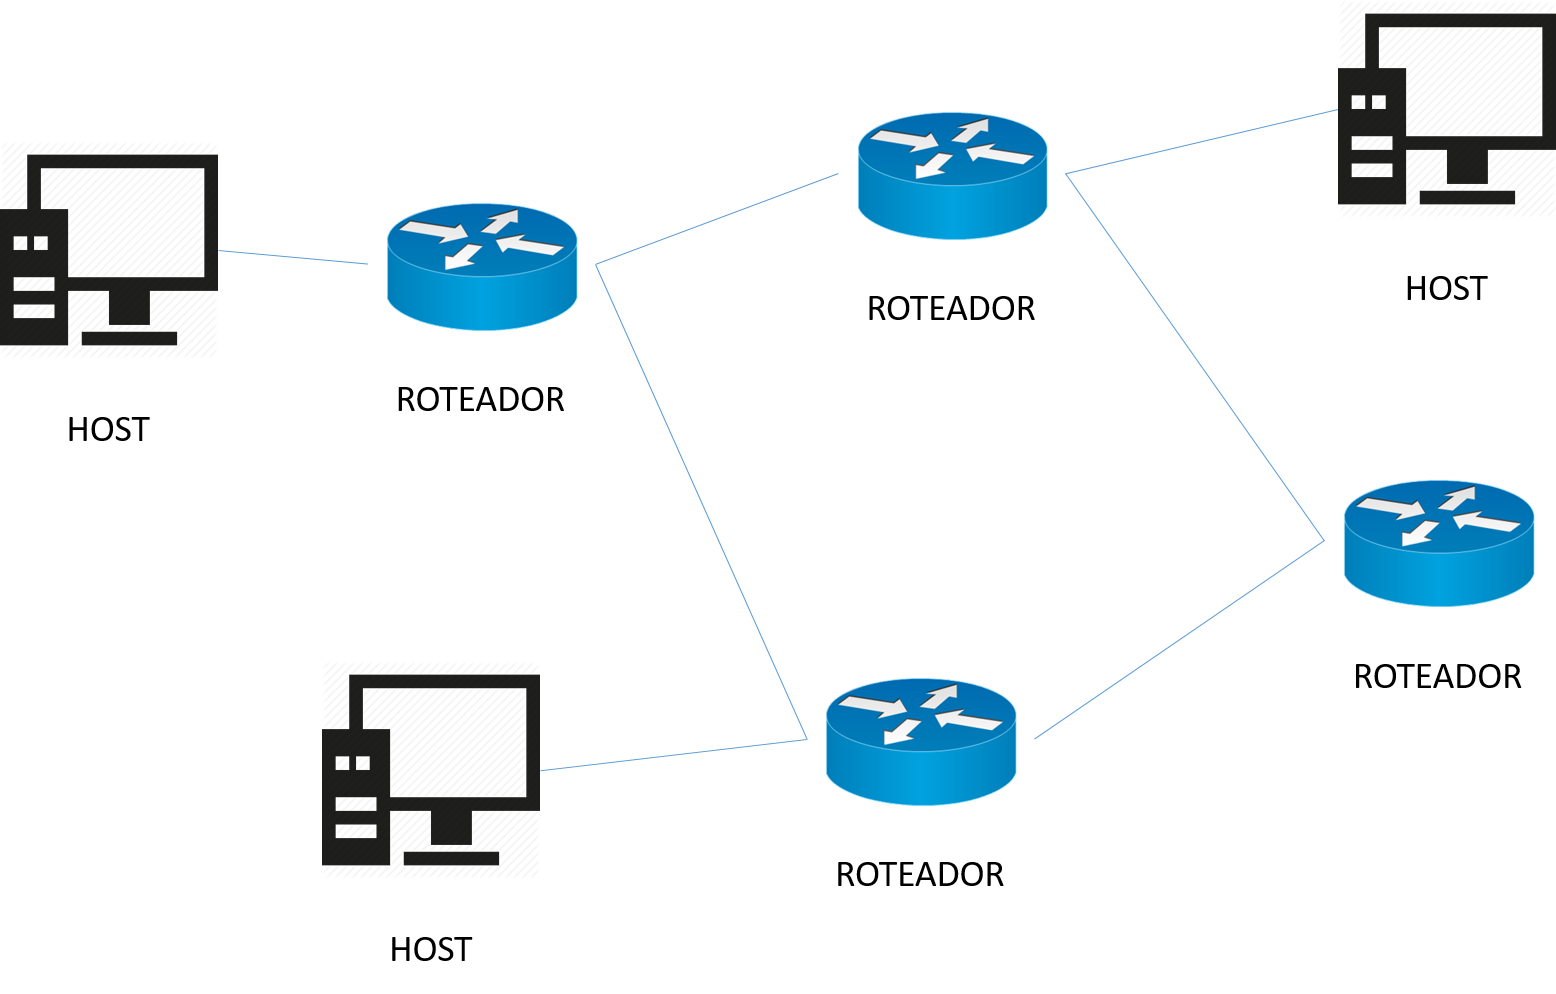
\includegraphics[width=0.7\textwidth]{Introducao/Rede.png}
\caption{Estrutura de uma Rede}
\label{Fig_Rede}
\end{figure}

Essa estrutura se mostrou extremamente eficiente, e permitiu que a expansão em nível mundial da Internet, uma vez que diversas redes com tamanhos e topologias diferentes conseguem se comunicar. 

Proporcional à expansão da Internet e a criação de cada vez mais dispositivos capazes de usá-la, houve um grande aumento no fluxo de dados. Tal aumento advém de práticas como o consumo de vídeo, através de plataformas como Youtube, Netflix, etc, sendo este o tipo de dado mais consumido e o segundo que mais cresce desde 2017\cite{CISCO}

Portanto, devido a essa progressiva demanda, novas arquiteturas de rede estão sendo investigadas. Contudo, como o núcleo da arquitetura atual, ou seja, os nós de comutação, são implementados via hardware, a implementação de arquiteturas experimentais se torna pouco viável, devido aos grandes custos dessa mudança de hardware, além do fato que essa troca iria interromper o fluxo de produção atual de uma rede, fator que dificulta o teste e validação de novas arquiteturas em ambientes reais, principalmente em redes de larga escala.

Dessa forma, soluções baseadas em software se tornaram mais atraentes devido a possibilidade de serem implementadas sem troca de hardware e sem interrupção da rede. Uma dessas alternativas que tem ganhado destaque é o paradigma SDN(Software Defined NetWork) juntamente com o protocolo OpenFlow. Uma rede SDN, utiliza de um dispositivo chamado controlador, que se conecta a todos os nós da rede, para configurá-los de acordo com o gerente da rede. O protocolo Openflow é um protocolo voltado para as redes SDN, que permite que o controlador se comunique com os comutatores.

A implementação de redes SDN ainda está numa fase experimental, e por isso, diversas pesquisas estão sendo desenvolvidas para verificar a performance desse tipo de rede. Uma das grandes vantagens de uma rede SDN é a possibilidade de separar o tráfego de dados em fluxos diferentes, além de poder alterar a tabela de encaminhamento dos comutatores para atingir um melhor desempenho da rede. 

Dessa forma, o objetivo desse trabalho é a criação de uma aplicação capaz de monitorar o fluxo de uma rede e identificar o consumo de dados de vídeos, provenientes de duas das principais plataformas de streaming : Youtube e NetFlix. Essa aplicação será integrada a um tipo de controlador chamado POX e testada através de software capaz de simular redes fisicas, chamado Mininet. Os conceitos de SDN , protocolo OpenFlow e controlador POX serão explicados de forma mais detalhada no capítulo 2.

\section{Objetivos}
\subsection{Objetivo geral}
Implementar e avaliar o desempenho de uma aplicação de monitoramento e classificação de fluxos de dados, utilizando uma rede SDN , junto com um controlador do tipo POX.

\subsection{Objetivos Específicos}

\begin{itemize}
\item Criar e configurar um ambiente de rede SDN, onde seja possível gerar e capturar todo o tráfego da rede. 
\item Implementar um módulo de monitoramento do tráfego da rede, para análise posterior.
\item Implementar o módulo de identificação e classificação do tipo de dados que trafega pela rede.
\item Implementar um módulo de detecção e tratamento de falhas na rede, para que a aplicação possa priorizar um determino tipo de fluxo.
\item Utilizar um banco da dados SQL, para armazenar todos os dados gerados pela aplicação
\end{itemize}3
\section{Estrutura do Trabalho}
Este trabalho será estruturado em 5 capítulos. No capítulo 2 serão explicados mais profundamente os conceitos de paradigma SDN, protoloco OpenFlow, controlador POX, além de das estruturas da arquitetura atual da Internet. Os módulos criados para a aplicação, suas funcionalidades, especificações, e ferramentas utilizadas serão apresentados no capitulo 3, assim como o ambiente em que o módulo foi testado.

O capítulo 4 será feita uma exposição e análise dos resultados obtidos. E por fim, no capítulo 5 serão expostas as conclusões, considerações finais e trabalhos futuros.




\documentclass[
	% -- opções da classe memoir --
	12pt,				% tamanho da fonte
	openright,			% capítulos começam em pág ímpar (insere página vazia caso preciso)
	twoside,			% para impressão em verso e anverso. Oposto a oneside
	a4paper,			% tamanho do papel. 
	% -- opções da classe abntex2 --
	%chapter=TITLE,		% títulos de capítulos convertidos em letras maiúsculas
	%section=TITLE,		% títulos de seções convertidos em letras maiúsculas
	%subsection=TITLE,	% títulos de subseções convertidos em letras maiúsculas
	%subsubsection=TITLE,% títulos de subsubseções convertidos em letras maiúsculas
	% -- opções do pacote babel --
	english,			% idioma adicional para hifenização
	french,				% idioma adicional para hifenização
	spanish,			% idioma adicional para hifenização
	brazil,				% o último idioma é o principal do documento
	]{abntex2}

\usepackage{cmap}			% Mapear caracteres especiais no PDF
\usepackage{lmodern}			% Usa a fonte Latin Modern			
\usepackage[T1]{fontenc}		% Selecao de codigos de fonte.
\usepackage[utf8]{inputenc}		% Codificacao do documento (conversão automática dos acentos)
\usepackage{lastpage}			% Usado pela Ficha catalográfica
\usepackage{indentfirst}		           % Indenta o primeiro parágrafo de cada seção.
\usepackage{color}				% Controle das cores
\usepackage{graphicx}			% Inclusão de gráficos
\usepackage{lipsum}			% para geração de dummy text

\usepackage[brazilian,hyperpageref]{backref}   % Paginas com as citações na bibl
\usepackage[alf]{abntex2cite}	                         % Citações padrão ABNT
% Configurações do pacote backref
% Usado sem a opção hyperpageref de backref
\renewcommand{\backrefpagesname}{Citado na(s) página(s):~}
% Texto padrão antes do número das páginas
\renewcommand{\backref}{}
% Define os textos da citação
\renewcommand*{\backrefalt}[4]{
	\ifcase #1 %
		Nenhuma citação no texto.%
	\or
		Citado na página #2.%
	\else
		Citado #1 vezes nas páginas #2.%
	\fi}%
% ---


% ---
% Informações de dados para CAPA e FOLHA DE ROSTO
% ---
\titulo{Modelo de Monografia de \\ Trabalho de Conclusão de Curso com \abnTeX}
\autor{<Nome Completo do Aluno>}
\local{Belo Horizonte}
\data{2013}
\orientador{Prof. <Nome Completo do Orientador>}
%\coorientador{Prof. }
\instituicao{%
  Universidade Federal de Minas Gerais -- UFMG
  \par
  Escola de Engenharia
  \par
  Curso de Graduação em Engenharia Elétrica}
\tipotrabalho{Trabalho de Conclusão de Curso}
% O preambulo deve conter o tipo do trabalho, o objetivo, o nome da instituição e a área de concentração 
\preambulo{Monografia apresentada durante o Seminário dos Trabalhos de Conclusão do Curso de Graduação em Engenharia Elétrica da UFMG, como parte dos requisitos necessários à obtenção do título de Engenheiro Eletricista.}
% alterando o aspecto da cor azul
\definecolor{blue}{RGB}{41,5,195}

% informações do PDF
\makeatletter
\hypersetup{
     	%pagebackref=true,
		pdftitle={\@title}, 
		pdfauthor={\@author},
    	pdfsubject={\imprimirpreambulo},
	    pdfcreator={LaTeX with abnTeX2},
		pdfkeywords={abnt}{latex}{abntex}{abntex2}{trabalho acadêmico}, 
		colorlinks=true,       	% false: boxed links; true: colored links
    	linkcolor=blue,          	           % color of internal links
    	citecolor=blue,        		% color of links to bibliography
    	filecolor=magenta,      		% color of file links
		urlcolor=blue,
		bookmarksdepth=4
}
\makeatother
% O tamanho do parágrafo é dado por:
\setlength{\parindent}{1.3cm}

% Controle do espaçamento entre um parágrafo e outro:
\setlength{\parskip}{0.2cm}  % tente também \onelineskip
\makeindex

% Início do documento
% ----
\begin{document}
% Retira espaço extra obsoleto entre as frases.
\frenchspacing 
%\imprimircapa
%\imprimirfolhaderosto

%\include{Inicio_Dedicatoria_resumo}

% ----------------------------------------------------------
% Capítulo 1 - Introdução
% ----------------------------------------------------------

\include{Introducao/main}
\include{Revisao/main}
\include{Metodologia/main}
% ----------------------------------------------------------
% Capítulo 2 - Revisão Bibliográfica
% ----------------------------------------------------------

% ----------------------------------------------------------
% Capítulo 3 - Metodologia
% ----------------------------------------------------------



% ----------------------------------------------------------
% Capítulo 4 - Resultados e Discussao
% ----------------------------------------------------------

% ----------------------------------------------------------
% Capítulo 5 - Conclusões
% ----------------------------------------------------------

% ---
% Finaliza a parte no bookmark do PDF, para que se inicie o bookmark na raiz
% ---
\bookmarksetup{startatroot}% 
% ---

% ----------------------------------------------------------
% ELEMENTOS PÓS-TEXTUAIS
% ----------------------------------------------------------
\postextual

% ----------------------------------------------------------
% Referências bibliográficas
% ----------------------------------------------------------
\bibliography{abntex2-modelo-references}

% ----------------------------------------------------------
% Apêndices
% ----------------------------------------------------------

% ---
% Inicia os apêndices
% ---
% \begin{apendicesenv}

% % Imprime uma página indicando o início dos apêndices
% \partapendices

% % ----------------------------------------------------------
% \chapter{Quisque libero justo}
% % ----------------------------------------------------------

% \lipsum[50-54]

% % ----------------------------------------------------------
% \chapter{Nullam elementum urna vel imperdiet sodales elit ipsum pharetra}
% % ----------------------------------------------------------
% \lipsum[55-59]

% \end{apendicesenv}
% % ---

% % ----------------------------------------------------------
% % Anexos
% % ----------------------------------------------------------

% % ---
% % Inicia os anexos
% % ---
% \begin{anexosenv}

% % Imprime uma página indicando o início dos anexos
% \partanexos
% % ---
% \chapter{Morbi ultrices rutrum lorem}
% % ---
% \lipsum[60]

% % ---
% \chapter{Cras non urna sed feugiat cum sociis natoque penatibus}
% % ---
% \lipsum[61-63]

% % ---
% \chapter{Fusce facilisis lacinia dui}
% % ---
% \lipsum[64-65]

% \end{anexosenv}

\end{document}

\documentclass[
	% -- opções da classe memoir --
	12pt,				% tamanho da fonte
	openright,			% capítulos começam em pág ímpar (insere página vazia caso preciso)
	twoside,			% para impressão em verso e anverso. Oposto a oneside
	a4paper,			% tamanho do papel. 
	% -- opções da classe abntex2 --
	%chapter=TITLE,		% títulos de capítulos convertidos em letras maiúsculas
	%section=TITLE,		% títulos de seções convertidos em letras maiúsculas
	%subsection=TITLE,	% títulos de subseções convertidos em letras maiúsculas
	%subsubsection=TITLE,% títulos de subsubseções convertidos em letras maiúsculas
	% -- opções do pacote babel --
	english,			% idioma adicional para hifenização
	french,				% idioma adicional para hifenização
	spanish,			% idioma adicional para hifenização
	brazil,				% o último idioma é o principal do documento
	]{abntex2}

\usepackage{cmap}			% Mapear caracteres especiais no PDF
\usepackage{lmodern}			% Usa a fonte Latin Modern			
\usepackage[T1]{fontenc}		% Selecao de codigos de fonte.
\usepackage[utf8]{inputenc}		% Codificacao do documento (conversão automática dos acentos)
\usepackage{lastpage}			% Usado pela Ficha catalográfica
\usepackage{indentfirst}		           % Indenta o primeiro parágrafo de cada seção.
\usepackage{color}				% Controle das cores
\usepackage{graphicx}			% Inclusão de gráficos
\usepackage{lipsum}			% para geração de dummy text

\usepackage[brazilian,hyperpageref]{backref}   % Paginas com as citações na bibl
\usepackage[alf]{abntex2cite}	                         % Citações padrão ABNT
% Configurações do pacote backref
% Usado sem a opção hyperpageref de backref
\renewcommand{\backrefpagesname}{Citado na(s) página(s):~}
% Texto padrão antes do número das páginas
\renewcommand{\backref}{}
% Define os textos da citação
\renewcommand*{\backrefalt}[4]{
	\ifcase #1 %
		Nenhuma citação no texto.%
	\or
		Citado na página #2.%
	\else
		Citado #1 vezes nas páginas #2.%
	\fi}%
% ---


% ---
% Informações de dados para CAPA e FOLHA DE ROSTO
% ---
\titulo{Modelo de Monografia de \\ Trabalho de Conclusão de Curso com \abnTeX}
\autor{<Nome Completo do Aluno>}
\local{Belo Horizonte}
\data{2013}
\orientador{Prof. <Nome Completo do Orientador>}
%\coorientador{Prof. }
\instituicao{%
  Universidade Federal de Minas Gerais -- UFMG
  \par
  Escola de Engenharia
  \par
  Curso de Graduação em Engenharia Elétrica}
\tipotrabalho{Trabalho de Conclusão de Curso}
% O preambulo deve conter o tipo do trabalho, o objetivo, o nome da instituição e a área de concentração 
\preambulo{Monografia apresentada durante o Seminário dos Trabalhos de Conclusão do Curso de Graduação em Engenharia Elétrica da UFMG, como parte dos requisitos necessários à obtenção do título de Engenheiro Eletricista.}
% alterando o aspecto da cor azul
\definecolor{blue}{RGB}{41,5,195}

% informações do PDF
\makeatletter
\hypersetup{
     	%pagebackref=true,
		pdftitle={\@title}, 
		pdfauthor={\@author},
    	pdfsubject={\imprimirpreambulo},
	    pdfcreator={LaTeX with abnTeX2},
		pdfkeywords={abnt}{latex}{abntex}{abntex2}{trabalho acadêmico}, 
		colorlinks=true,       	% false: boxed links; true: colored links
    	linkcolor=blue,          	           % color of internal links
    	citecolor=blue,        		% color of links to bibliography
    	filecolor=magenta,      		% color of file links
		urlcolor=blue,
		bookmarksdepth=4
}
\makeatother
% O tamanho do parágrafo é dado por:
\setlength{\parindent}{1.3cm}

% Controle do espaçamento entre um parágrafo e outro:
\setlength{\parskip}{0.2cm}  % tente também \onelineskip
\makeindex

% Início do documento
% ----
\begin{document}
% Retira espaço extra obsoleto entre as frases.
\frenchspacing 
%\imprimircapa
%\imprimirfolhaderosto

%\include{Inicio_Dedicatoria_resumo}

% ----------------------------------------------------------
% Capítulo 1 - Introdução
% ----------------------------------------------------------

\include{Introducao/main}
\include{Revisao/main}
\include{Metodologia/main}
% ----------------------------------------------------------
% Capítulo 2 - Revisão Bibliográfica
% ----------------------------------------------------------

% ----------------------------------------------------------
% Capítulo 3 - Metodologia
% ----------------------------------------------------------



% ----------------------------------------------------------
% Capítulo 4 - Resultados e Discussao
% ----------------------------------------------------------

% ----------------------------------------------------------
% Capítulo 5 - Conclusões
% ----------------------------------------------------------

% ---
% Finaliza a parte no bookmark do PDF, para que se inicie o bookmark na raiz
% ---
\bookmarksetup{startatroot}% 
% ---

% ----------------------------------------------------------
% ELEMENTOS PÓS-TEXTUAIS
% ----------------------------------------------------------
\postextual

% ----------------------------------------------------------
% Referências bibliográficas
% ----------------------------------------------------------
\bibliography{abntex2-modelo-references}

% ----------------------------------------------------------
% Apêndices
% ----------------------------------------------------------

% ---
% Inicia os apêndices
% ---
% \begin{apendicesenv}

% % Imprime uma página indicando o início dos apêndices
% \partapendices

% % ----------------------------------------------------------
% \chapter{Quisque libero justo}
% % ----------------------------------------------------------

% \lipsum[50-54]

% % ----------------------------------------------------------
% \chapter{Nullam elementum urna vel imperdiet sodales elit ipsum pharetra}
% % ----------------------------------------------------------
% \lipsum[55-59]

% \end{apendicesenv}
% % ---

% % ----------------------------------------------------------
% % Anexos
% % ----------------------------------------------------------

% % ---
% % Inicia os anexos
% % ---
% \begin{anexosenv}

% % Imprime uma página indicando o início dos anexos
% \partanexos
% % ---
% \chapter{Morbi ultrices rutrum lorem}
% % ---
% \lipsum[60]

% % ---
% \chapter{Cras non urna sed feugiat cum sociis natoque penatibus}
% % ---
% \lipsum[61-63]

% % ---
% \chapter{Fusce facilisis lacinia dui}
% % ---
% \lipsum[64-65]

% \end{anexosenv}

\end{document}
% ----------------------------------------------------------
% Capítulo 2 - Revisão Bibliográfica
% ----------------------------------------------------------

% ----------------------------------------------------------
% Capítulo 3 - Metodologia
% ----------------------------------------------------------



% ----------------------------------------------------------
% Capítulo 4 - Resultados e Discussao
% ----------------------------------------------------------

% ----------------------------------------------------------
% Capítulo 5 - Conclusões
% ----------------------------------------------------------

% ---
% Finaliza a parte no bookmark do PDF, para que se inicie o bookmark na raiz
% ---
\bookmarksetup{startatroot}% 
% ---

% ----------------------------------------------------------
% ELEMENTOS PÓS-TEXTUAIS
% ----------------------------------------------------------
\postextual

% ----------------------------------------------------------
% Referências bibliográficas
% ----------------------------------------------------------
\bibliography{abntex2-modelo-references}

% ----------------------------------------------------------
% Apêndices
% ----------------------------------------------------------

% ---
% Inicia os apêndices
% ---
% \begin{apendicesenv}

% % Imprime uma página indicando o início dos apêndices
% \partapendices

% % ----------------------------------------------------------
% \chapter{Quisque libero justo}
% % ----------------------------------------------------------

% \lipsum[50-54]

% % ----------------------------------------------------------
% \chapter{Nullam elementum urna vel imperdiet sodales elit ipsum pharetra}
% % ----------------------------------------------------------
% \lipsum[55-59]

% \end{apendicesenv}
% % ---

% % ----------------------------------------------------------
% % Anexos
% % ----------------------------------------------------------

% % ---
% % Inicia os anexos
% % ---
% \begin{anexosenv}

% % Imprime uma página indicando o início dos anexos
% \partanexos
% % ---
% \chapter{Morbi ultrices rutrum lorem}
% % ---
% \lipsum[60]

% % ---
% \chapter{Cras non urna sed feugiat cum sociis natoque penatibus}
% % ---
% \lipsum[61-63]

% % ---
% \chapter{Fusce facilisis lacinia dui}
% % ---
% \lipsum[64-65]

% \end{anexosenv}

\end{document}
% ----------------------------------------------------------
% Capítulo 2 - Revisão Bibliográfica
% ----------------------------------------------------------

% ----------------------------------------------------------
% Capítulo 3 - Metodologia
% ----------------------------------------------------------



% ----------------------------------------------------------
% Capítulo 4 - Resultados e Discussao
% ----------------------------------------------------------

% ----------------------------------------------------------
% Capítulo 5 - Conclusões
% ----------------------------------------------------------

% ---
% Finaliza a parte no bookmark do PDF, para que se inicie o bookmark na raiz
% ---
\bookmarksetup{startatroot}% 
% ---

% ----------------------------------------------------------
% ELEMENTOS PÓS-TEXTUAIS
% ----------------------------------------------------------
\postextual

% ----------------------------------------------------------
% Referências bibliográficas
% ----------------------------------------------------------
\bibliography{abntex2-modelo-references}

% ----------------------------------------------------------
% Apêndices
% ----------------------------------------------------------

% ---
% Inicia os apêndices
% ---
% \begin{apendicesenv}

% % Imprime uma página indicando o início dos apêndices
% \partapendices

% % ----------------------------------------------------------
% \chapter{Quisque libero justo}
% % ----------------------------------------------------------

% \lipsum[50-54]

% % ----------------------------------------------------------
% \chapter{Nullam elementum urna vel imperdiet sodales elit ipsum pharetra}
% % ----------------------------------------------------------
% \lipsum[55-59]

% \end{apendicesenv}
% % ---

% % ----------------------------------------------------------
% % Anexos
% % ----------------------------------------------------------

% % ---
% % Inicia os anexos
% % ---
% \begin{anexosenv}

% % Imprime uma página indicando o início dos anexos
% \partanexos
% % ---
% \chapter{Morbi ultrices rutrum lorem}
% % ---
% \lipsum[60]

% % ---
% \chapter{Cras non urna sed feugiat cum sociis natoque penatibus}
% % ---
% \lipsum[61-63]

% % ---
% \chapter{Fusce facilisis lacinia dui}
% % ---
% \lipsum[64-65]

% \end{anexosenv}

\end{document}
% ----------------------------------------------------------
% Capítulo 2 - Revisão Bibliográfica
% ----------------------------------------------------------

% ----------------------------------------------------------
% Capítulo 3 - Metodologia
% ----------------------------------------------------------



% ----------------------------------------------------------
% Capítulo 4 - Resultados e Discussao
% ----------------------------------------------------------

% ----------------------------------------------------------
% Capítulo 5 - Conclusões
% ----------------------------------------------------------

% ---
% Finaliza a parte no bookmark do PDF, para que se inicie o bookmark na raiz
% ---
\bookmarksetup{startatroot}% 
% ---

% ----------------------------------------------------------
% ELEMENTOS PÓS-TEXTUAIS
% ----------------------------------------------------------
\postextual

% ----------------------------------------------------------
% Referências bibliográficas
% ----------------------------------------------------------
\bibliography{abntex2-modelo-references}

% ----------------------------------------------------------
% Apêndices
% ----------------------------------------------------------

% ---
% Inicia os apêndices
% ---
% \begin{apendicesenv}

% % Imprime uma página indicando o início dos apêndices
% \partapendices

% % ----------------------------------------------------------
% \chapter{Quisque libero justo}
% % ----------------------------------------------------------

% \lipsum[50-54]

% % ----------------------------------------------------------
% \chapter{Nullam elementum urna vel imperdiet sodales elit ipsum pharetra}
% % ----------------------------------------------------------
% \lipsum[55-59]

% \end{apendicesenv}
% % ---

% % ----------------------------------------------------------
% % Anexos
% % ----------------------------------------------------------

% % ---
% % Inicia os anexos
% % ---
% \begin{anexosenv}

% % Imprime uma página indicando o início dos anexos
% \partanexos
% % ---
% \chapter{Morbi ultrices rutrum lorem}
% % ---
% \lipsum[60]

% % ---
% \chapter{Cras non urna sed feugiat cum sociis natoque penatibus}
% % ---
% \lipsum[61-63]

% % ---
% \chapter{Fusce facilisis lacinia dui}
% % ---
% \lipsum[64-65]

% \end{anexosenv}

\end{document}